\documentclass[]{spie}
\usepackage[]{graphicx}
\usepackage{url}
\usepackage[]{amsmath}
\usepackage{subcaption}



\title{Efficient illuminant correction in the Local, Linear, Learned ({\LARGE$\boldsymbol L^3$}) method}

\author{Francois G. Germain\supit{a}, Iretiayo A. Akinola\supit{b}, Qiyuan Tian\supit{b}, Steven Lansel\supit{c}, and Brian A. Wandell\supit{b,d}
\skiplinehalf
\supit{a}Center for Computer Research in Music and Acoustics,\\ Stanford University, Stanford, CA-94305, USA;\\
\supit{b}Electrical Engineering Department, Stanford University, Stanford, CA-94305, USA;\\
\supit{c}Olympus Corporation of the Americas, Sunnyvale, CA-94085, USA;\\
\supit{d}Psychology Department, Stanford University, Stanford, CA-94305, USA.
}

\authorinfo{Send correspondence to Francois G. Germain. E-mail: FG (fgermain@stanford.edu), IA (iakinola@stanford.edu), QT (qytian@stanford.edu), SL (steven.lansel@olympus.com), BW (wandell@stanford.edu)}

\begin{document}
\maketitle

\begin{abstract}

To speed the development of novel camera architectures, we proposed a method,  $L^3$  (Local, Linear and Learned), that uses camera simulation to create an optimized image processing pipeline. The $L^3$  method assigns each pixel into one of about 400 classes and uses camera simulation and machine learning to derive a linear transform for the data in each class.  The linear transform maps the sensor data at the pixel and its neighborhood into the target output space (e.g., CIE XYZ).  In the original implementation, illuminant correction was achieved by training with sensor data acquired under one illuminant (illuminant-acquisition) and selecting transforms that optimize the rendering into a standard illuminant (e.g., D65-rendered). This approach requires storing illuminant-dependent transforms, and each table of transforms can be relatively large. Here, we show that the table derived from D65-acquisition to D65-rendered can serve as an illuminant-independent table that converts sensor data from any illuminant (illuminant-acquisition) to calibrated XYZ data under the same illuminant (illuminant-rendered). To perform illuminant correction, we propose that the image processing pipeline applies that table to the sensor data, and then follows with a simple color correction transform applied to the illuminant-rendered XYZ data. The mean color reproduction error between the illuminant-independent table and the true XYZ is on the order of 4$\Delta E$  units (max $\sim 13 \Delta E$), which is comparable to the error in the multiple table approach. The single table approach reduces storage requirements significantly without substantially  degrading color reproduction accuracy.


\end{abstract}

\keywords{Local Linear Learned ($L^3$), image processing pipeline, illuminant correction }

\section{INTRODUCTION}

The $L^3$ algorithm automatically generates a standard image processing pipeline (sensor correction, demosaicking, illuminant correction, noise reduction) for novel camera architectures  [1-4]. The standard image processing pipeline comprises two parts. First, the pipeline classifies each pixel (based on a statistical analysis of the responses at the pixel and its neighborhood) into one of many possible classes [1].  Second, the processing pipeline linearly transforms the data of the pixel and its neighborhood to the target output space.  The $L^3$ algorithm selects optimal parameters for the pipeline given a specific sensor and camera architecture. 
The classes are defined by the user and the linear transforms for each class are derived through a training process.  The selection of the transforms rely on an accurate camera software simulation; we used the Image Systems Engineering Toolbox (ISET) simulation software [5, 6]. The simulation converts many samples of natural scenes to sensor data. The desired rendering, i.e. CIE XYZ values for consumer photography, are computed from the known natural scene radiance. The $L^3$ algorithm learns linear filters that convert the sensor data in each class to the CIE XYZ values. 

\begin{figure}
\begin{center}
    \includegraphics[height=7cm]{illuminant_processing}
\end{center}
\caption{ (a) Cross-illuminant (XI) illuminant-dependent $L^3$ processing. (b) Same-illuminant (SI) illuminant-independent L3 processing  followed by a linear color correction transform (T).}
\label{fig:sensordisplay}
\end{figure}

\section{MOTIVATION: ILLUMINANT CORRECTION}

Illuminant correction is an essential part of the image processing pipeline that is necessary to account for the perceptual phenomenon of color constancy [7]. The visual system adapts to changes in the ambient light level and color, and this adaptation has the general effect of preserving the color appearance of an object (e.g. a white shirt) across conditions (sunlight to tungsten light). Because the human visual system adapts to the illuminant, to preserve color appearance the linear transforms in $L^3$  method used for rendering must adapt, too. 

In the original algorithm, we anticipated selecting classes and learning a table of linear transforms for each illumination condition (cross-illuminant, Figure 1a).  These cross-illuminant tables would be stored and applied for rendering. This approach pays a significant cost in computation and storage [1]. Hence, we explore an alternative approach that separates illuminant correction from the rest of the pipeline. In this approach, we learn a same-illuminant table, that renders data acquired under one illuminant into XYZ values under the same illuminant.  This accomplishes demosaicking, denoising and sensor correction, but it does not perform illuminant correction (Figure 1b). We then apply an illuminant correction transform to obtain the final rendering. This architecture requires training and storing only one table of $L^3$ transforms and one illuminant correction matrix for each illuminant of interest. 

\section{METHOD}

\textit{General simulation conditions}. We used ISET [5,6] to simulate digital camera processing. The ISET camera model includes the simulation of scene radiance, optics, sensor electronics and image processing pipeline (here the $L^3$ pipeline). In this report, we model the camera as an f/4 lens with diffraction limited optics and focal length of 3mm. The sensor uses a RGB/W color filter array (CFA) layout described in [1], with parameter values as in Figure 2.  

The table of $L^3$ filters is learned from simulated data of natural scenes following the process described in [1].  The $L^3$ algorithm uses simulated training data to learn a set of linear transforms. Each pixel in the simulated sensor data is assigned to a distinct class based on (a) its color (R, G, B, W and so forth), (b) the neighborhood light level (low, middle, high voltage), and (c) the neighborhood spatial structure (uniform or textured).  The transform for a given class is derived by optimizing a Wiener filter between the data in the pixel neighborhood in the sensor, and the corresponding ideal value in the target color space (XYZ). 

The rendering process identifies the class membership for each pixel in the sensor data and then applies the appropriate stored linear transform. The image processing pipeline, which performs demosaicking, denoising, sensor conversion is simply the application of these precomputed local, linear transforms. 

\textit{Learning the cross-illuminant tables.} Cross-illuminant (XI) tables of $L^3$ transforms are learned by simulating the sensor data under each test illuminant (D65, tungsten and fluorescent) and rendering to a target representation (XYZ) under a D65 illuminant. 

\textit{Learning the same-illuminant table.}  Same-illuminant (SI) tables of $L^3$ transforms are learned by simulating sensor data and the target display XYZ values using the same illuminant. We learned same-illuminant tables for D65, Tungsten, Fluorescent. To complete the rendering, we apply an illuminant correction transform from the acquisition illuminant to the final D65 rendering.  The matrix T is derived by a linear regression between the XYZ values in the acquired and target (D65) representations.  T is derived from first principles and is not dependent on the camera structure or $L^3$. 

In principle, any of the same-illuminant tables can be used in the SI approach. In fact, it is possible to learn a same-illuminant table using sensor data from an ensemble of illuminants. (e.g., a mixture of D65 and tungsten scenes). The linear transforms reflect the properties of the multiple illuminants used in the ensemble, rather than the requirements of a specific illuminant.  For example, the response level of a blue pixel under tungsten illuminant is typically quite low.  This is learned in the training and $L^3$ compensates by using linear transforms with more blurring compared to the D65 same-illuminant transform. We learned tables for two ensembles comprising data from a mixture of D65 and Tungsten illuminants and all three illuminants.

\textbf{Color evaluation:} To compare the different algorithms, we used data from hyperspectral scenes and simulated test charts.

\textit{Multispectral scenes.} We used a small set of multispectral scenes including the Macbeth (Gretag) color chart, fruits, and people.  These images compare the algorithms visually. 

\textit{Natural-100 reflectance chart.} To generate a systematic and quantitative assessment of the color reproduction error, we created a Natural-100 test chart (Figure 2). The chart includes 100 samples with natural object reflectances from five categories [XX], and a 10-sample gray color strip. The reflectances are grouped by category (20 food, 20 clothes, 20 nature, 5 hair, 15 skin and 20 paint color samples). To select the category samples we calculated 7 principal components for the entire set of natural reflectances, represented each sample by its component weights, and then formed clusters of the samples.  If N samples are needed from a category, we formed N clusters for that category and chose one sample from each cluster. By selecting one sample per cluster per category we ensure that the final chart has variety of reflectances that span the sample pool.

We compared the same-illuminant and cross-illuminant methods by measuring the color reproduction error.  This was measured in CIE2000 ΔΕ units [8] by comparing the ideal rendered XYZ display data under a D65 illuminant with the rendered data using the different $L^3$ tables.

\begin{figure}
 \begin{center}
\begin{minipage}{0.45\textwidth}
\begin{flushright}
 \begin{scriptsize}
\begin{tabular}{|l|c|}
\hline 
\multicolumn{2}{|c|}{\textbf{Optics(diffraction-limited)}} \\\hline 
Focal length(mm) & 3 \\  
F-number & 4 \\  
Aperture diameter (mm) & 0.75 \\ \hline 
\multicolumn{2}{|c|}{\textbf{Sensor}} \\ \hline 
Rows/Columns & 204 $\times$ 240 \\  
Size (mm) & 0.4488 $\times$ 0.528 \\  
Dark noise nonuniformity (mV) & 1.41 \\  
Photoreceptor nonuniformity (\% ) & $2.218 \times 10 ^{-3}$ \\  
Analog gain & 1 \\\hline 
\multicolumn{2}{|c|}{\textbf{Sensor pixel }} \\ \hline 
Width/height $(\mu V/e)$ & 200 \\  
Fill factor & 0.45  \\
Dark voltage (V/sec) & $1 \times 10^{-5}$ \\  
Read noise (mV) & 1.34 \\  
Conversion gain $(\mu V/e)$ & 200 \\  
Voltage swing (V) & 1.8 \\  
Well capacity (electrons) & 9000 \\ \hline 
\end{tabular} 
\end{scriptsize}
\end{flushright}
\end{minipage}\hfill
\begin{minipage}{0.45\textwidth}
\begin{flushleft}
 
\includegraphics[height=6cm]{natureBasedChart}
\end{flushleft}
\end{minipage}
\caption{Sensor parameter values (left) and Natural-100 color test chart (right)}

\label{fig:natureBasedChart}
\end{center}
\end{figure}



\section{EXPERIMENTAL RESULTS}

First, we compared the SI\_D65 and SI\_Tun tables in order to assess the suitability of SI\_D65 as illuminant-independent within-illuminant table (as presented in Figure 1b). The optimized filter weights differ slightly between the illuminant conditions. For example, under tungsten illuminant conditions the blue pixel data are generally noisier than the corresponding classes with D65 illumination. Consequently, the optimal filters weights sum more broadly over the blue pixels in the tungsten filters than in the D65 filters.

Even though the derived tables differ, for color reproduction error the rendering differences are rather small.  This can be seen by comparing Figure 3b and 3c which show the same camera data rendered with the SI\_D65 and SI\_Tun tables respectively derived from D65 and tungsten illumination. We use SI\_D65 as reference illuminant-independent within-illuminant table in the rest of the paper. 


\begin{figure}
\begin{center}
\begin{subfigure}[b]{0.3\textwidth}
    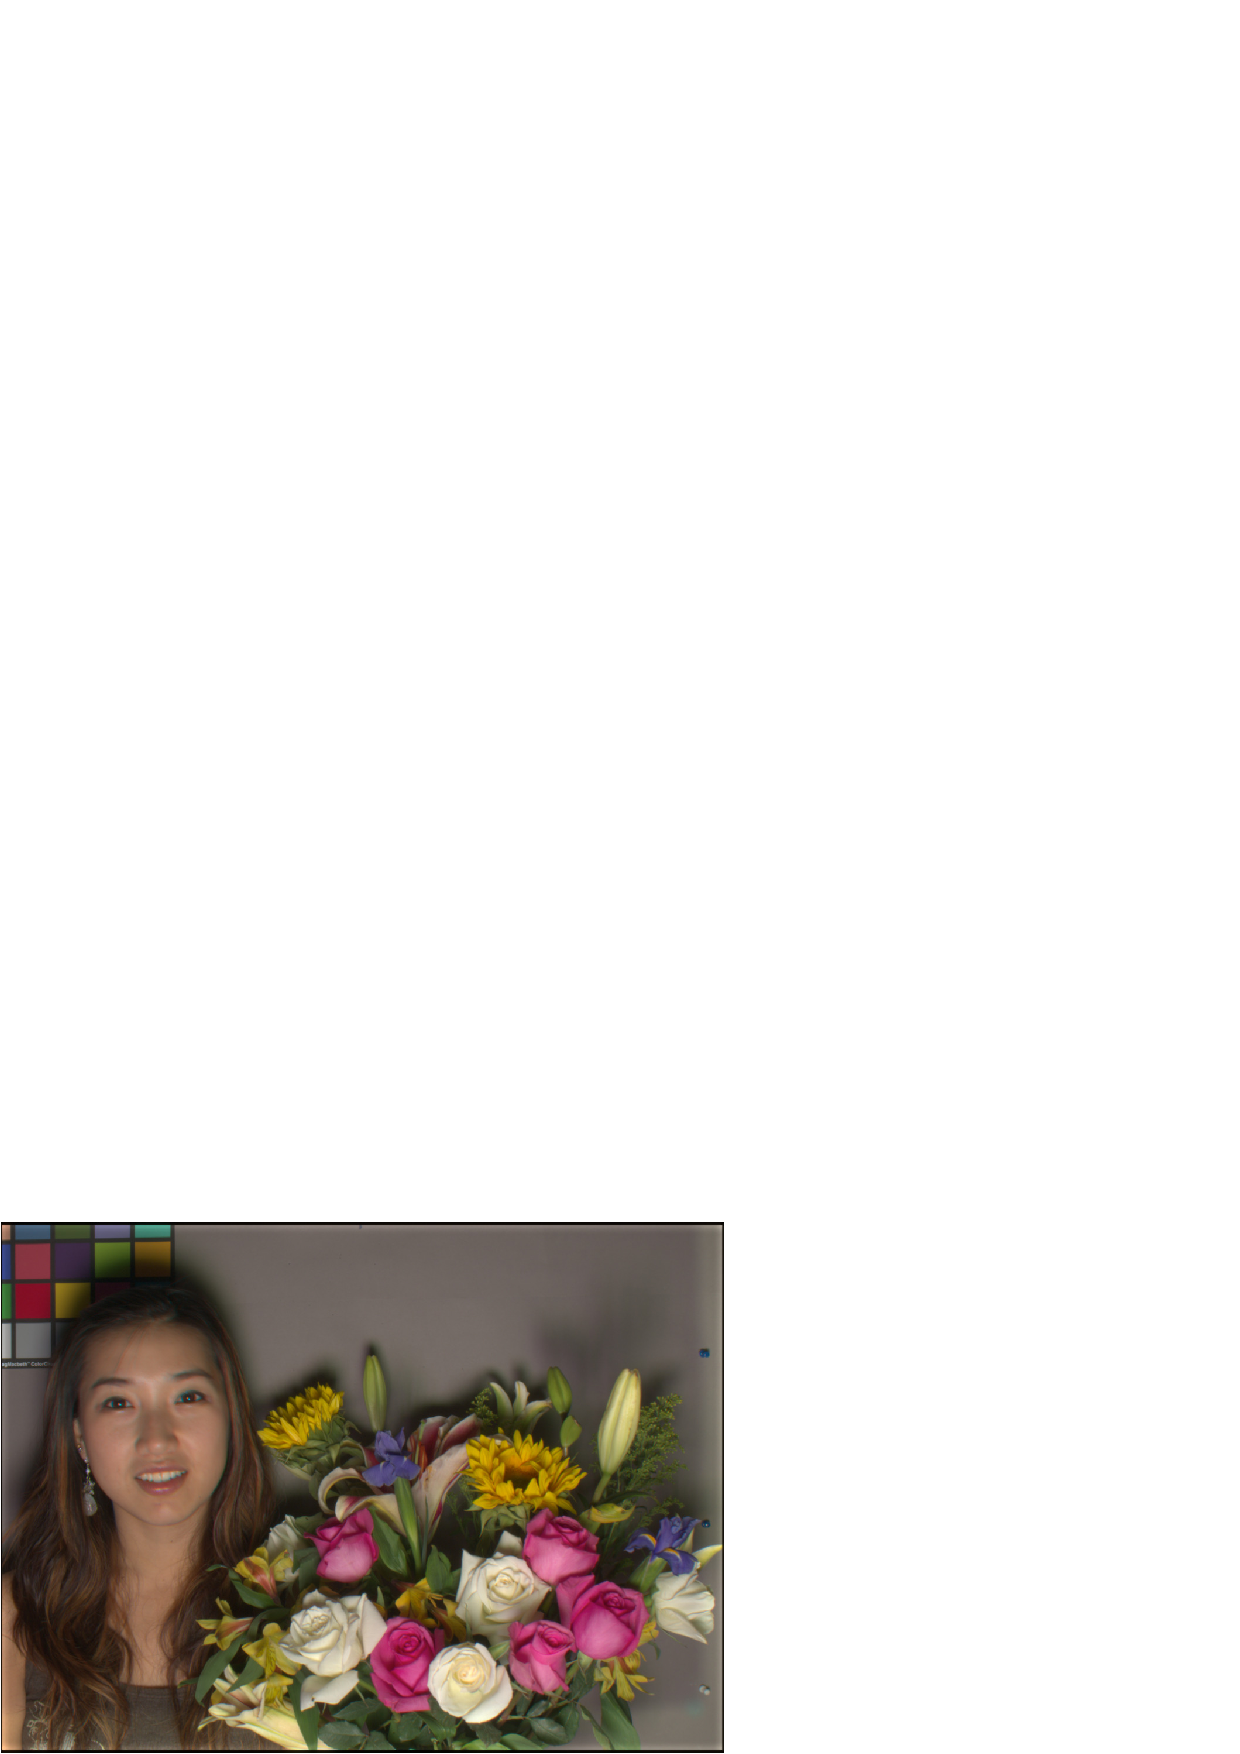
\includegraphics[width=\textwidth]{FaceId}
    
\includegraphics[width=\textwidth]{VeggieId}
    \caption{Ideal}
\end{subfigure}
\begin{subfigure}[b]{0.3\textwidth}
    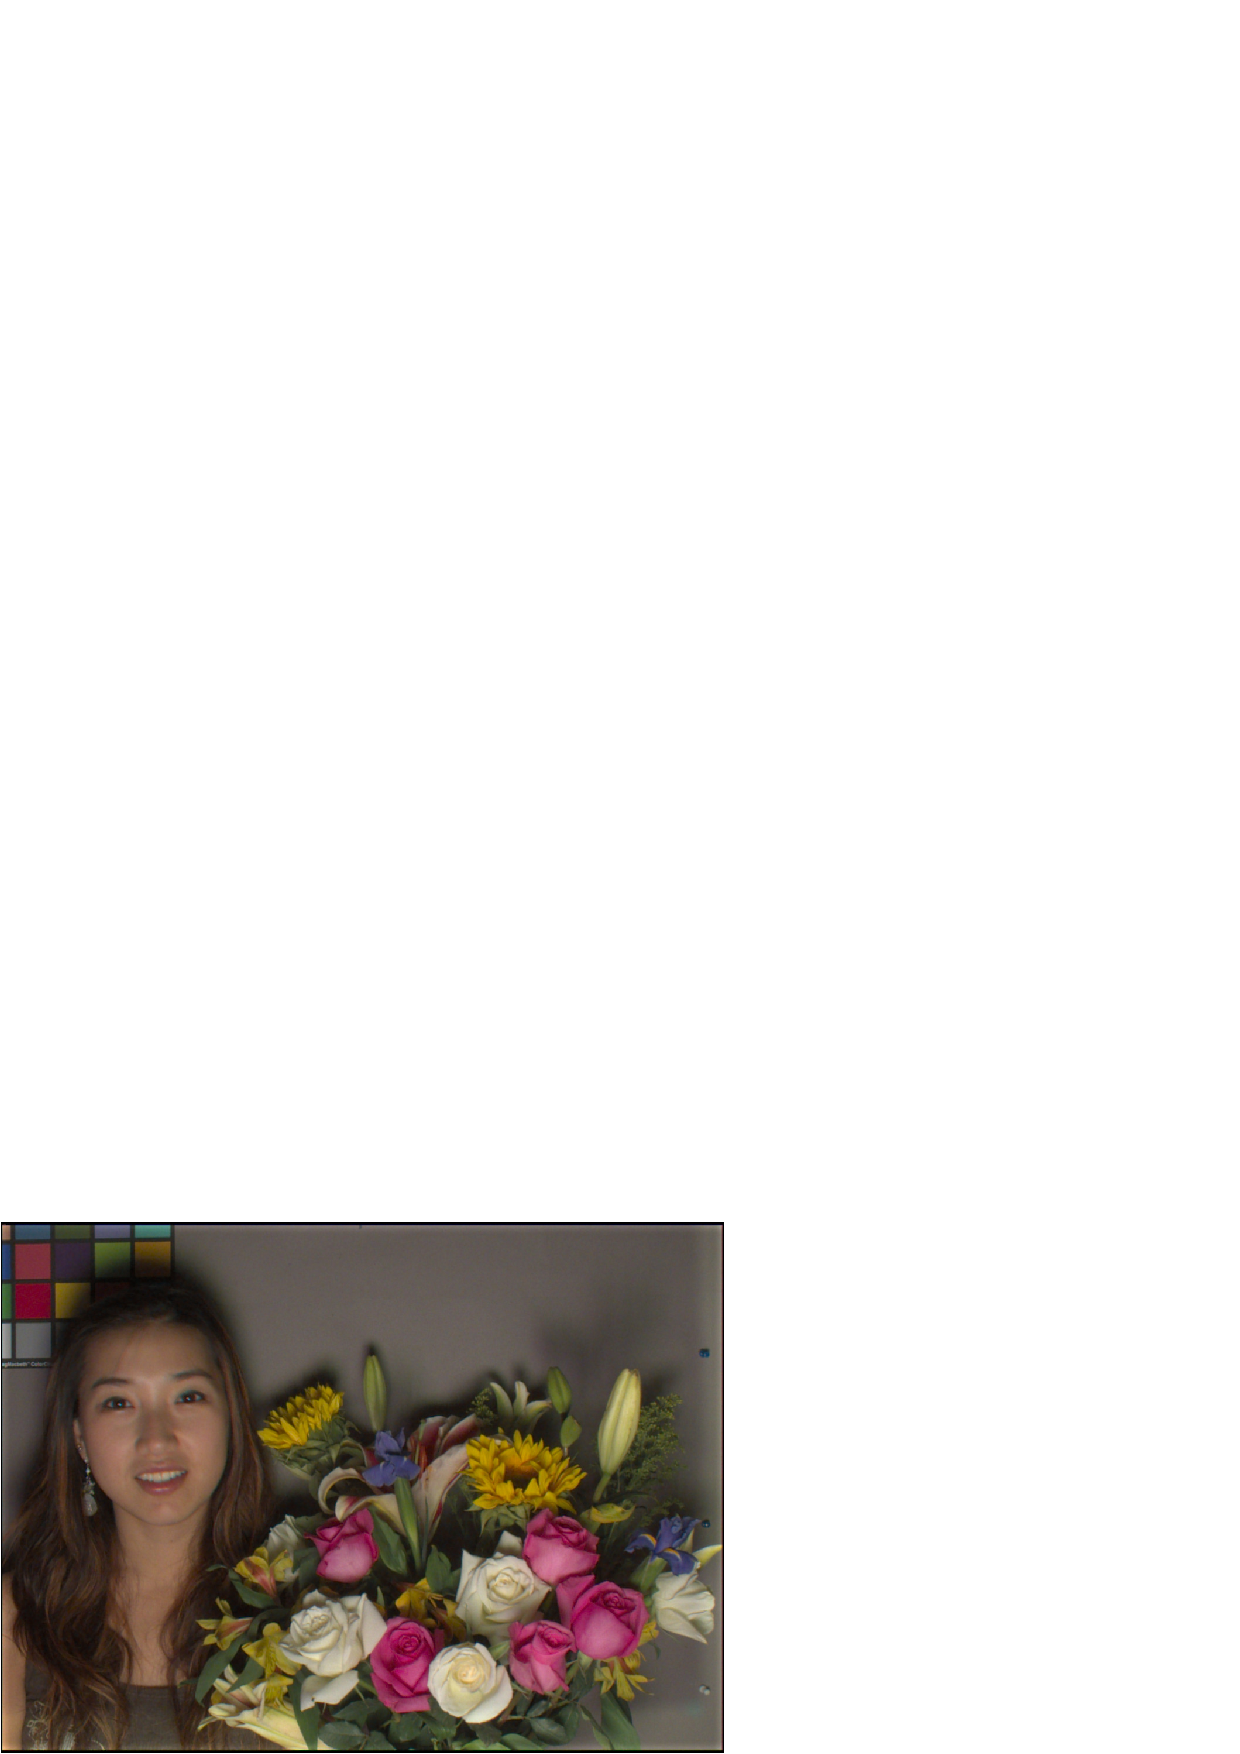
\includegraphics[width=\textwidth]{FaceTunXI}
    
\includegraphics[width=\textwidth]{VeggieTunXI}
    \caption{XI}
\end{subfigure}
\begin{subfigure}[b]{0.3\textwidth}
    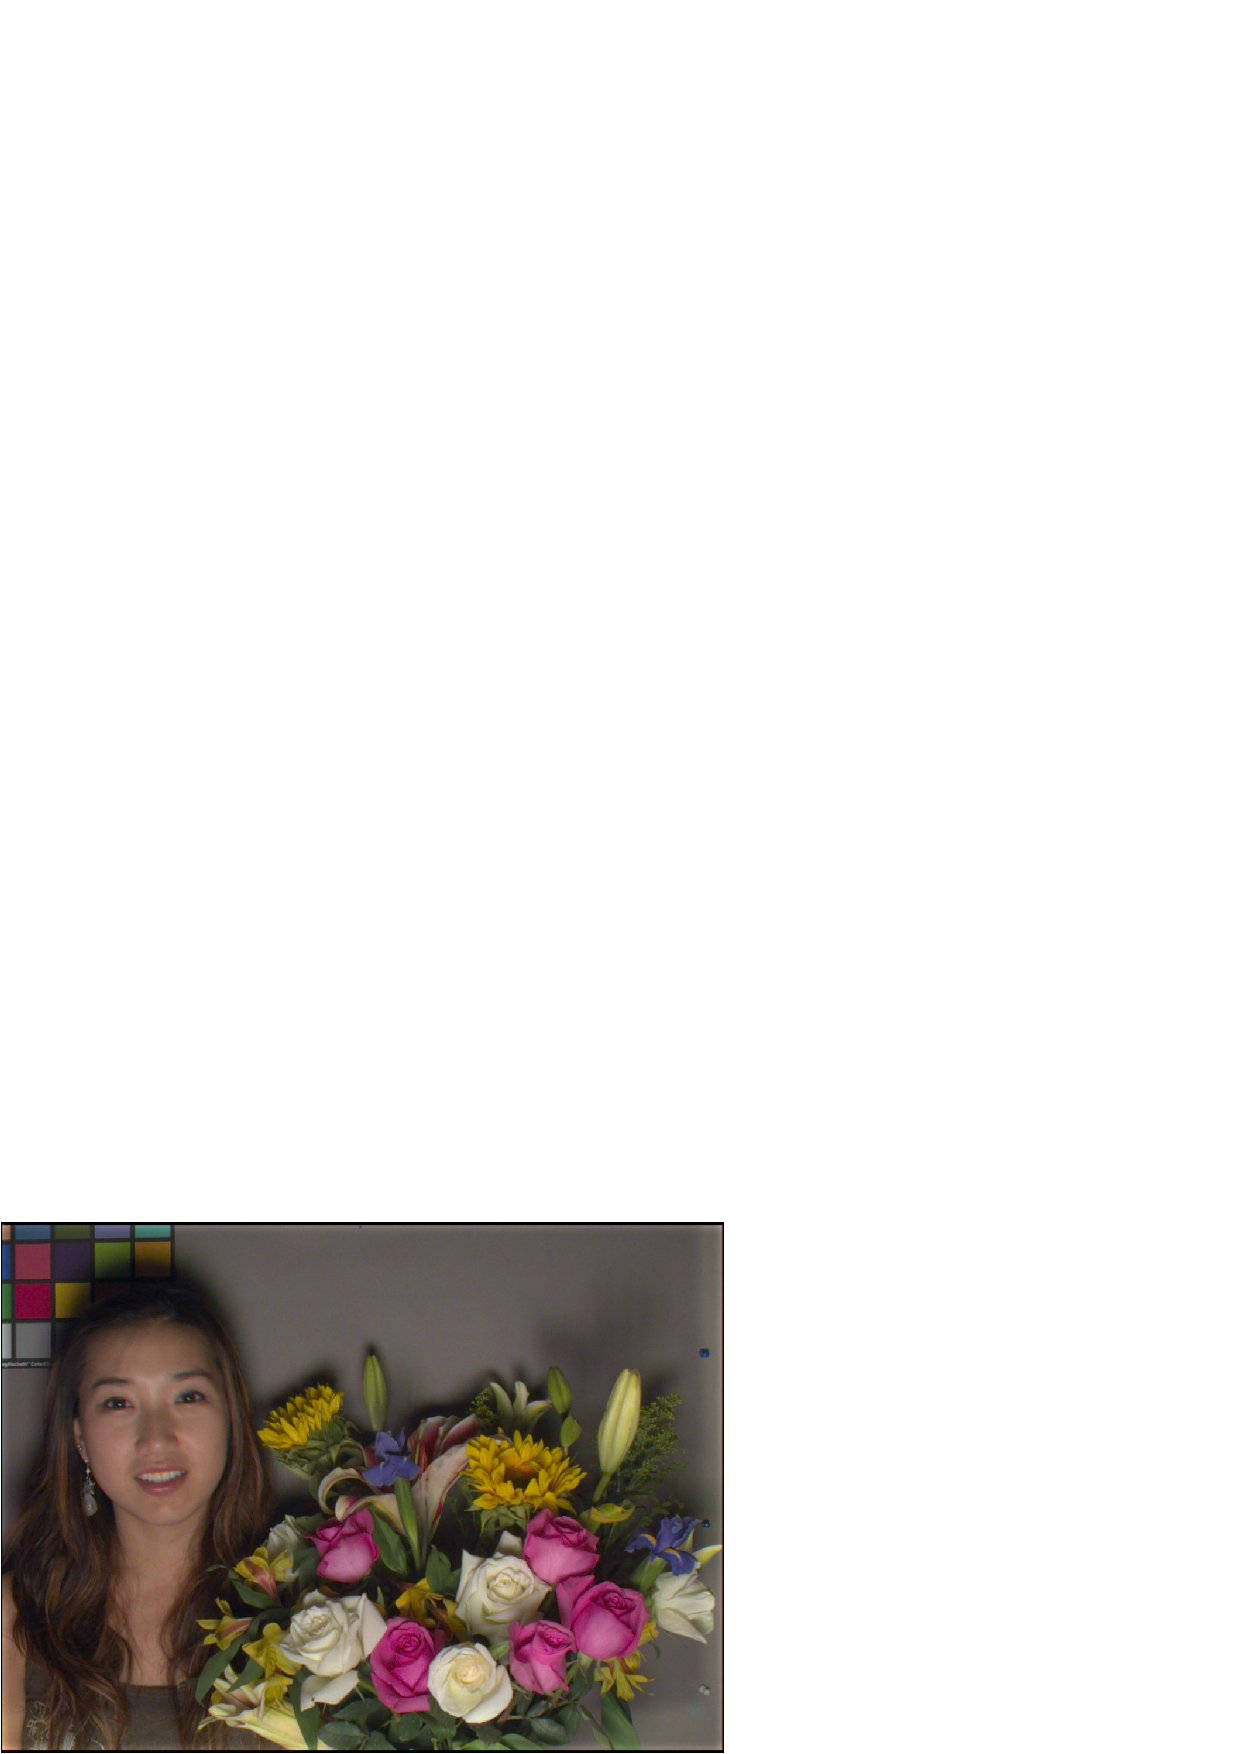
\includegraphics[width=\textwidth]{FaceTunSI}
    
\includegraphics[width=\textwidth]{VeggieTunSI}
    \caption{SI\_D65+T}
\end{subfigure}
\end{center}
\caption{\textbf{Cross-illuminant and same-illuminant algorithms perform equally well in color rendering for a tungsten illuminant.} (a) The ideal image under a D65 illumination. (b) A cross-illuminant analysis for the same image but acquired under a tungsten light. The L3 table was built from the tungsten-acquisition data and XYZ target values for a D65-rendered image. (c) A same-illuminant rendering.  In this case the  L3  table was built using the D65-acquisition data and target values for a D65-rendered image.  The final rendering combined the L3  table  and an illuminant correction matrix T in XYZ space. The cross-illuminant and same-illuminant architectures produce similar images in this case and in general.}
\label{fig:filters}
\end{figure}

\begin{figure}
\begin{center}
\begin{subfigure}[b]{0.3\textwidth}
    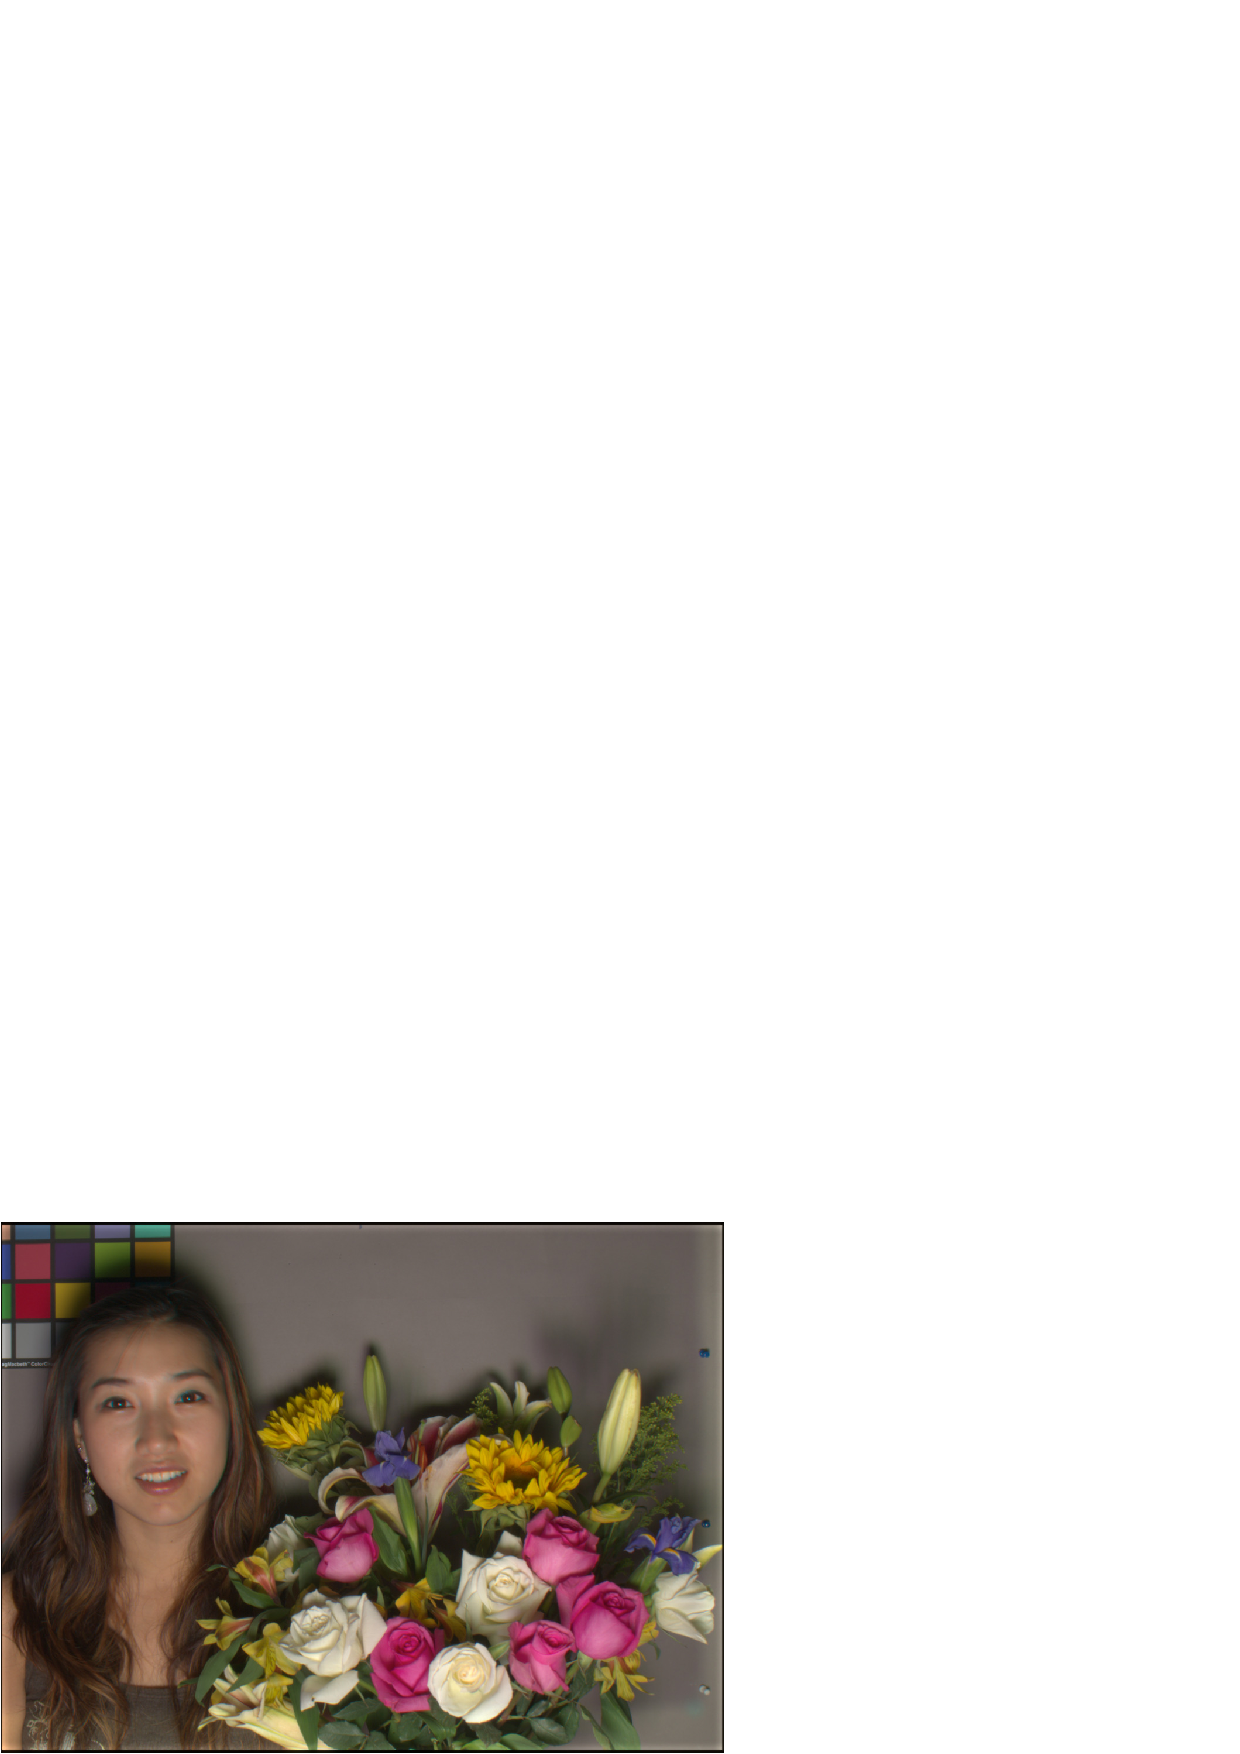
\includegraphics[width=\textwidth]{FaceId}
    
\includegraphics[width=\textwidth]{VeggieId}
    \caption{Ideal}
\end{subfigure}
\begin{subfigure}[b]{0.3\textwidth}
    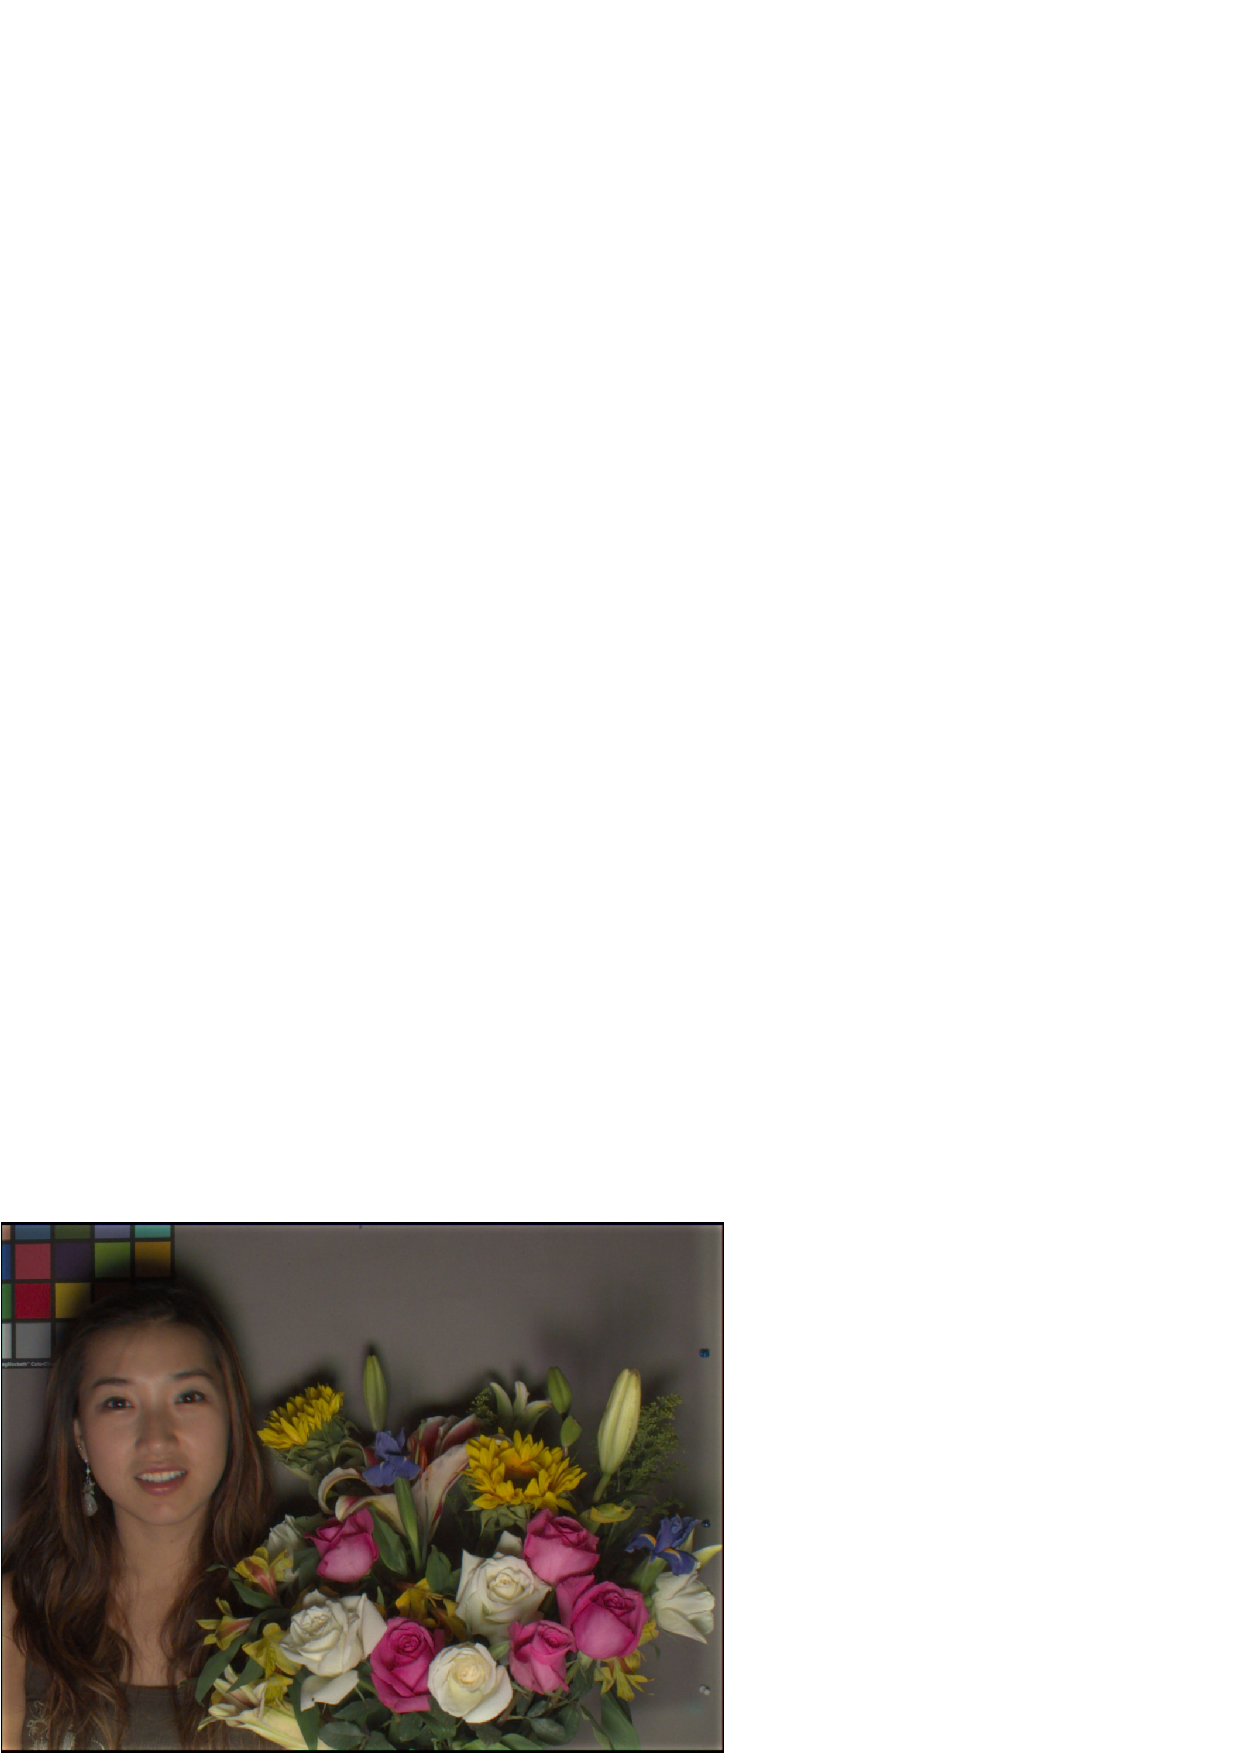
\includegraphics[width=\textwidth]{FaceFluXI}
    
\includegraphics[width=\textwidth]{VeggieFluXI}
    \caption{XI}
\end{subfigure}
\begin{subfigure}[b]{0.3\textwidth}
    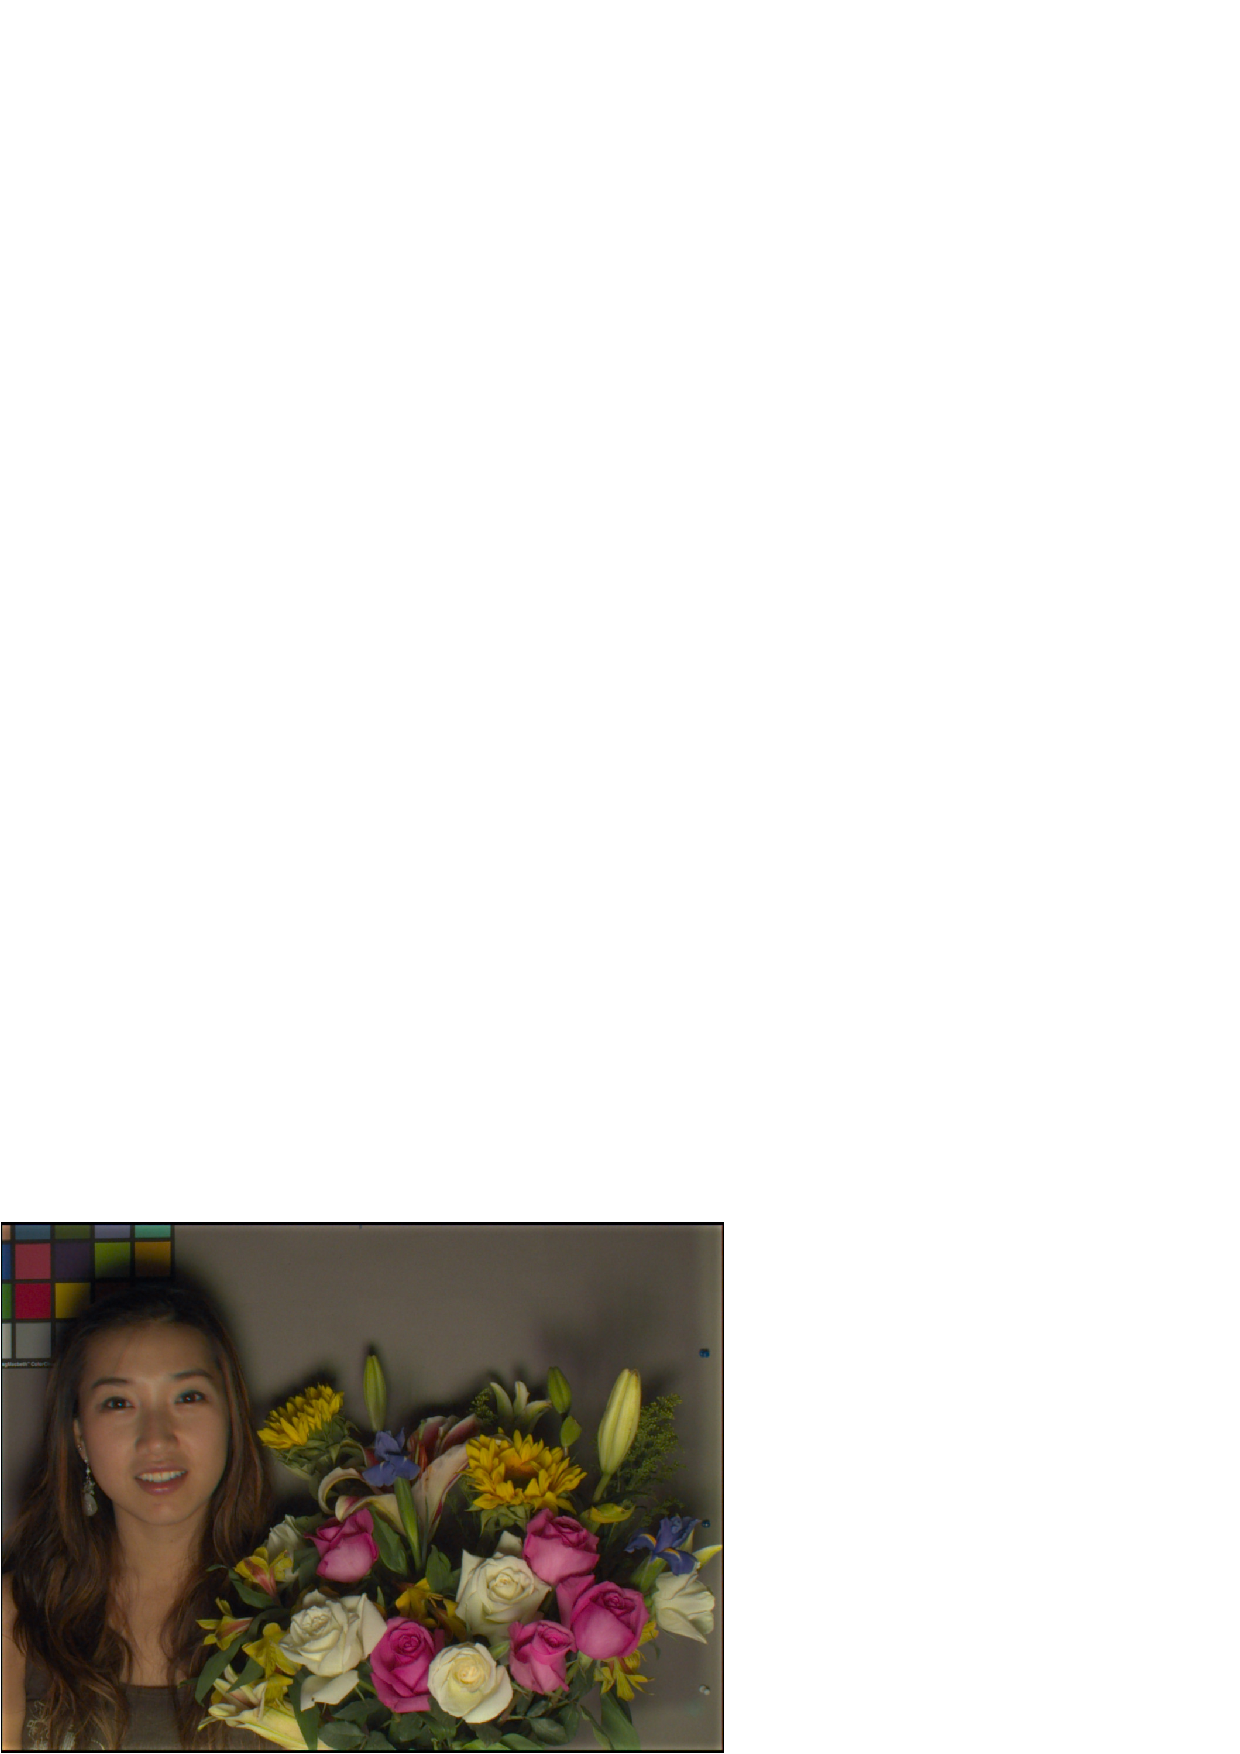
\includegraphics[width=\textwidth]{FaceFluSI}
    
\includegraphics[width=\textwidth]{VeggieFluSI}
    \caption{SI\_D65+T}
\end{subfigure}
\end{center}
\caption{\textbf{Cross-illuminant and same-illuminant algorithms perform equally well in color rendering for a fluorescent illuminant.} (a) The ideal image under a D65 illumination. (b) A cross-illuminant analysis for the same image but acquired under a fluorescent light. The L3 table was built from the fluorescent-acquisition data and XYZ target values for a D65-rendered image. (c) A same-illuminant rendering.  In this case the  L3  table was built using the D65-acquisition data and target values for a D65-rendered image.  The final rendering combined the L3  table  and an illuminant correction matrix T in XYZ space. The cross-illuminant and same-illuminant architectures produce similar images in this case and in general.}
\label{fig:filters}
\end{figure}


Second, we compared renderings using the illuminant-independent table (here SI\_D65) followed by a linear transformation T for illuminant correction in XYZ space (SI\_D65+T) with renderings using the cross-illuminant table (XI) between a tungsten illuminant and D65 target output (Figure 4).

We quantified the color rendering differences between the XI, SI\_Tun+T and SI\_D65+T  pipelines using the Natural-100 test chart by comparing the XYZ values with those of the ideal XYZ values (these are known because the data are simulated).  The color reproduction errors in the XI condition are identical to those in the SI\_Tun+T condition, while they are slightly smaller than those in the SI\_D65+T condition, indicating that color reproduction accuracy is mostly affected by the replacement of SI\_Tun by the illuminant-independent table (here SI\_D65).  However, the differences do not appear to be very significant for most consumer applications (Table 1). 


\begin {table}[H]
\begin{center}
\begin{tabular}{|l|c|c|}
\hline 
Color reproduction error ($\Delta E$) & Average (Std. dev.) & 90th percentile \\ \hline 
XI $L^3$ & 2.2 (1.8) & 4.2 \\  
SI\_Tun $L^3$ with linear color transform T (SI\_Tun+T) & 2.2 (1.8) & 4.2 \\  
SI\_D65 $L^3$ with linear color transform T (SI\_D65+T) & 3.6 (2.4) & 6.5 \\
SI\_E1 $L^3$ with linear color transform T (SI\_E1+T) & 2.6 (1.9) & 5.2 \\
SI\_E2 $L^3$ with linear color transform T (SI\_E2+T) & 4.0 (2.3) & 6.9 \\\hline 
\end{tabular} 
\end{center}\caption {Color reproduction errors (ΔE) for the Natural-100 color chart with illuminant correction from tungsten to D65 for the cross-illuminant table XI and several same-illuminant table followed by an illuminant correction matrix} 
\label{tab:colorErrorTable} 

\end{table}

\begin{figure}
\begin{subfigure}[b]{0.325\textwidth}
    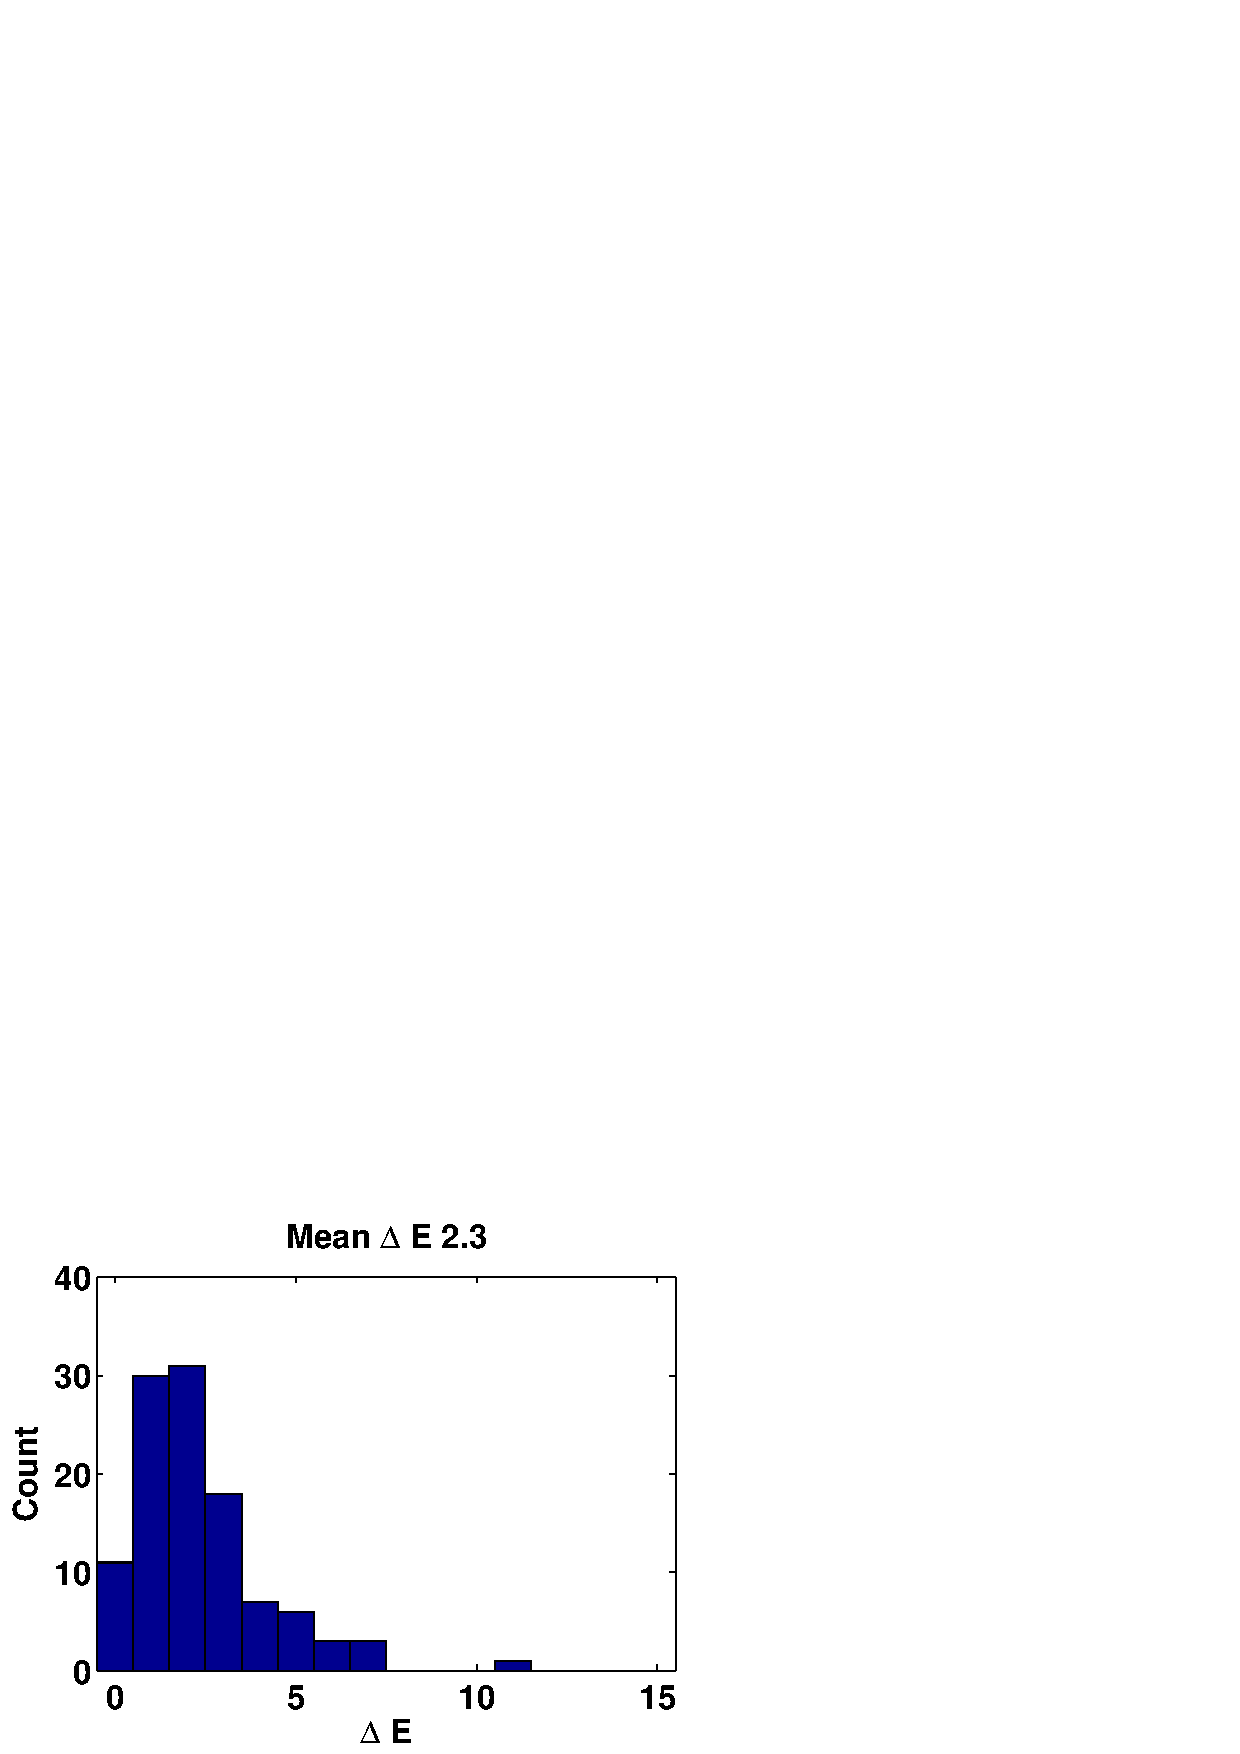
\includegraphics[width=\textwidth]{Hist_XI}
    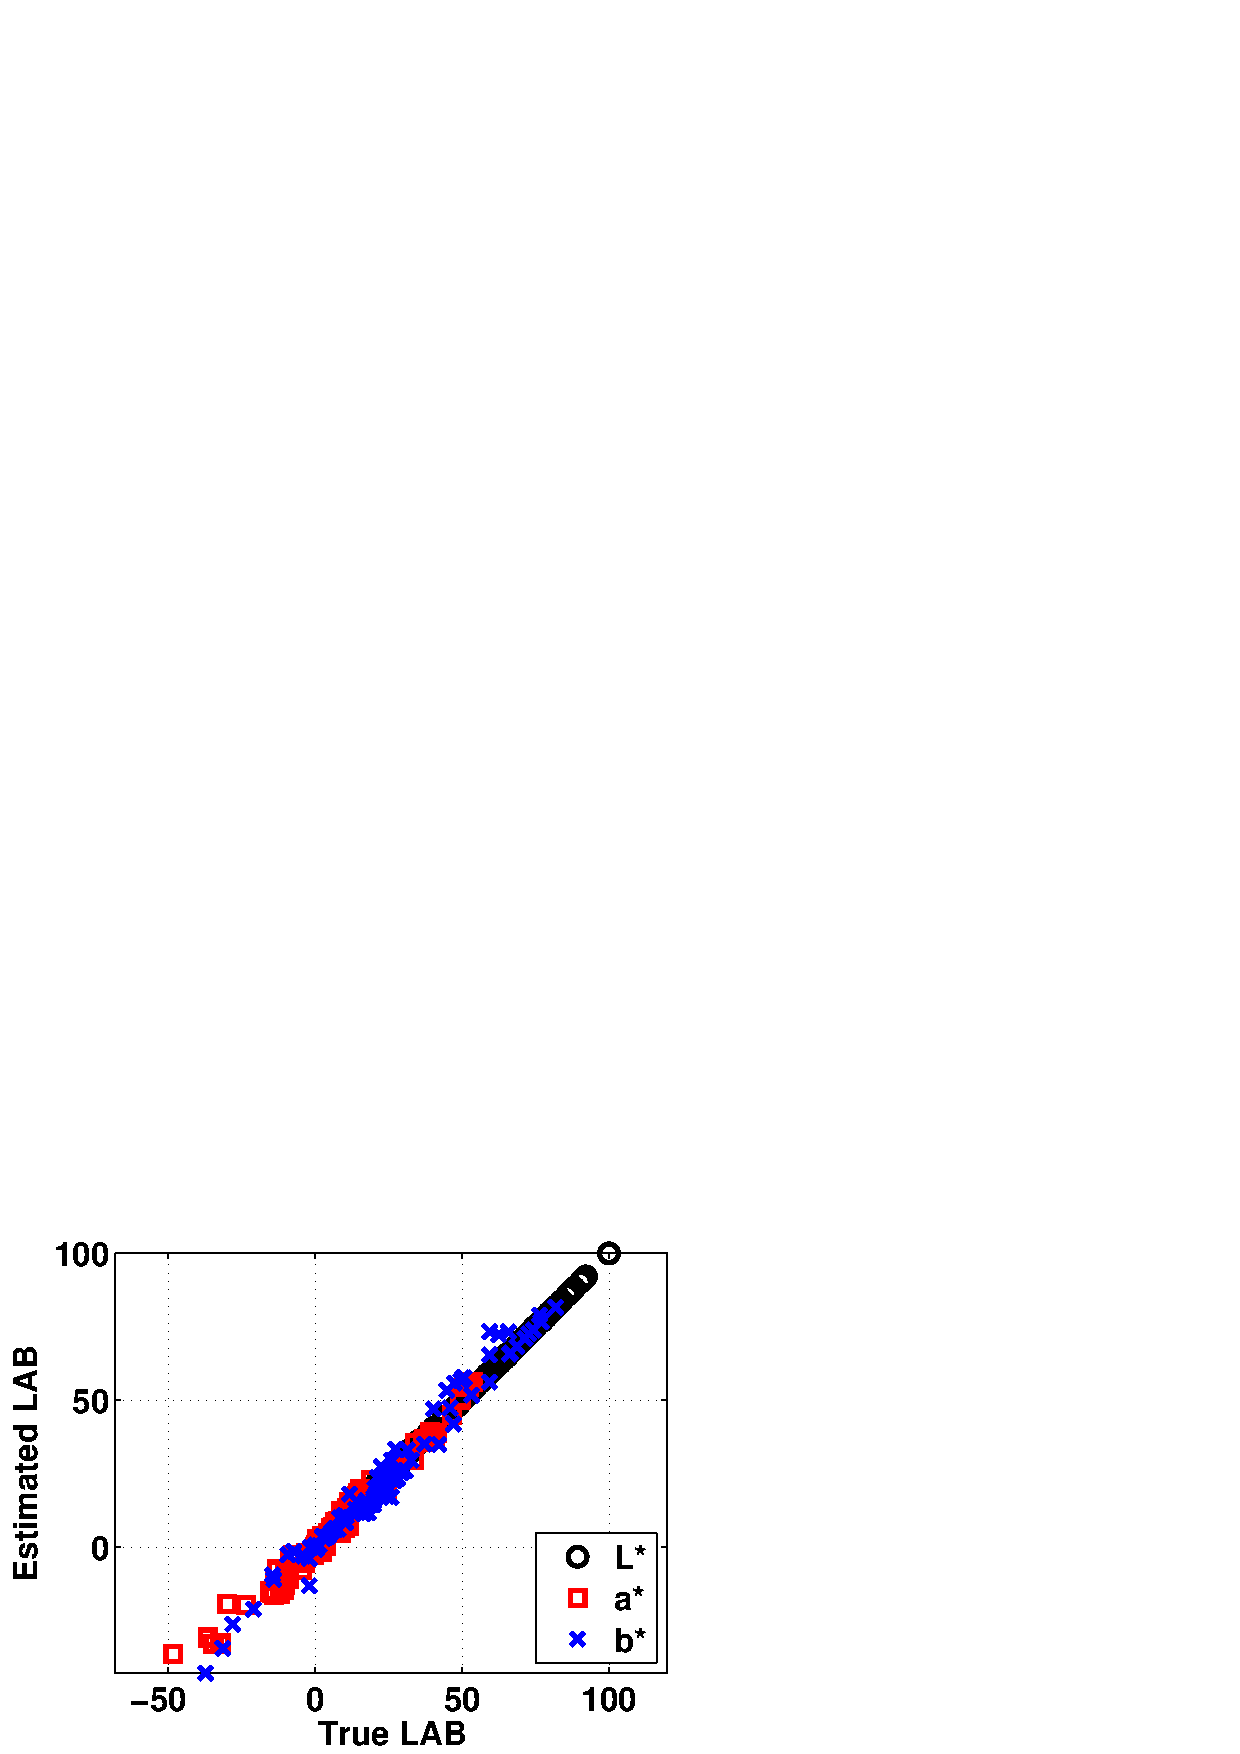
\includegraphics[width=\textwidth]{DeltaE_XI}
    \caption{XI}
\end{subfigure}
\begin{subfigure}[b]{0.325\textwidth}
    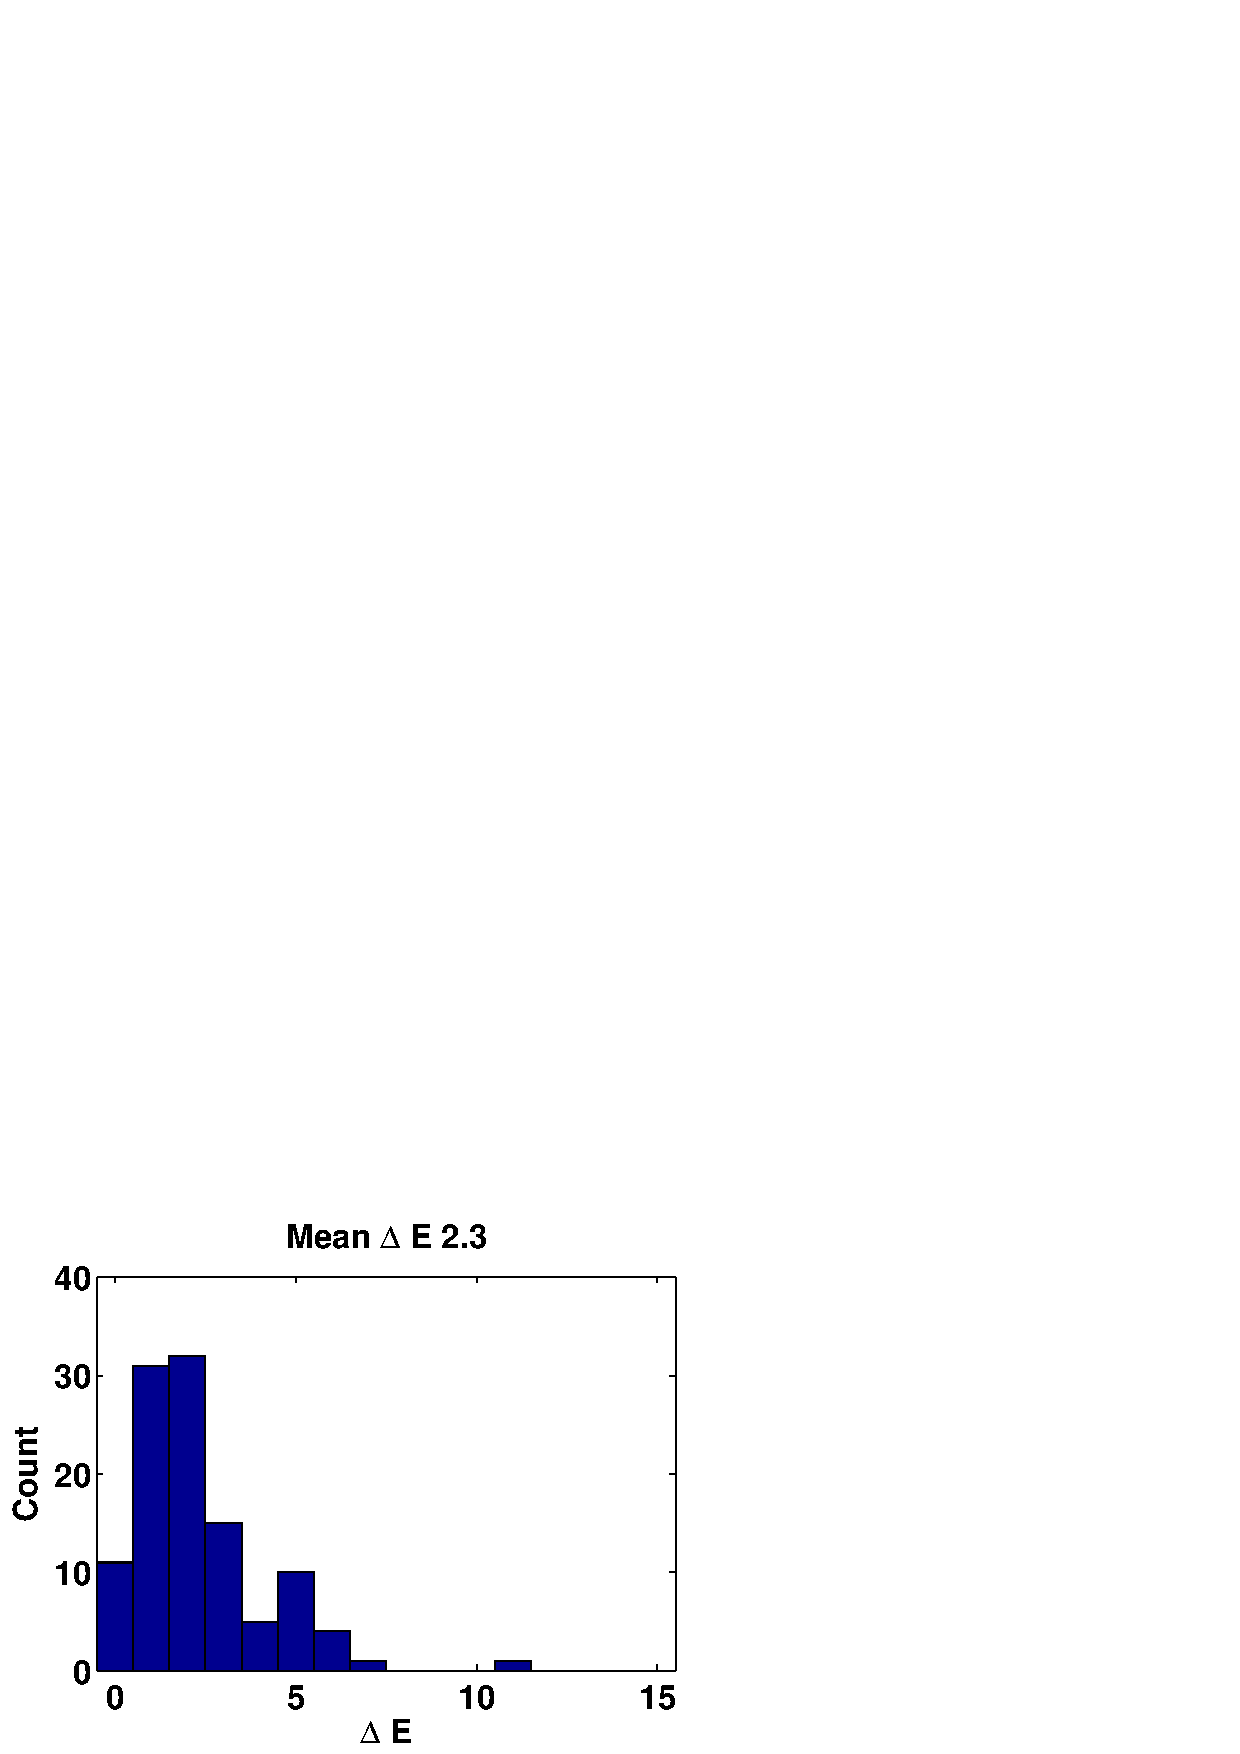
\includegraphics[width=\textwidth]{Hist_Tun}
    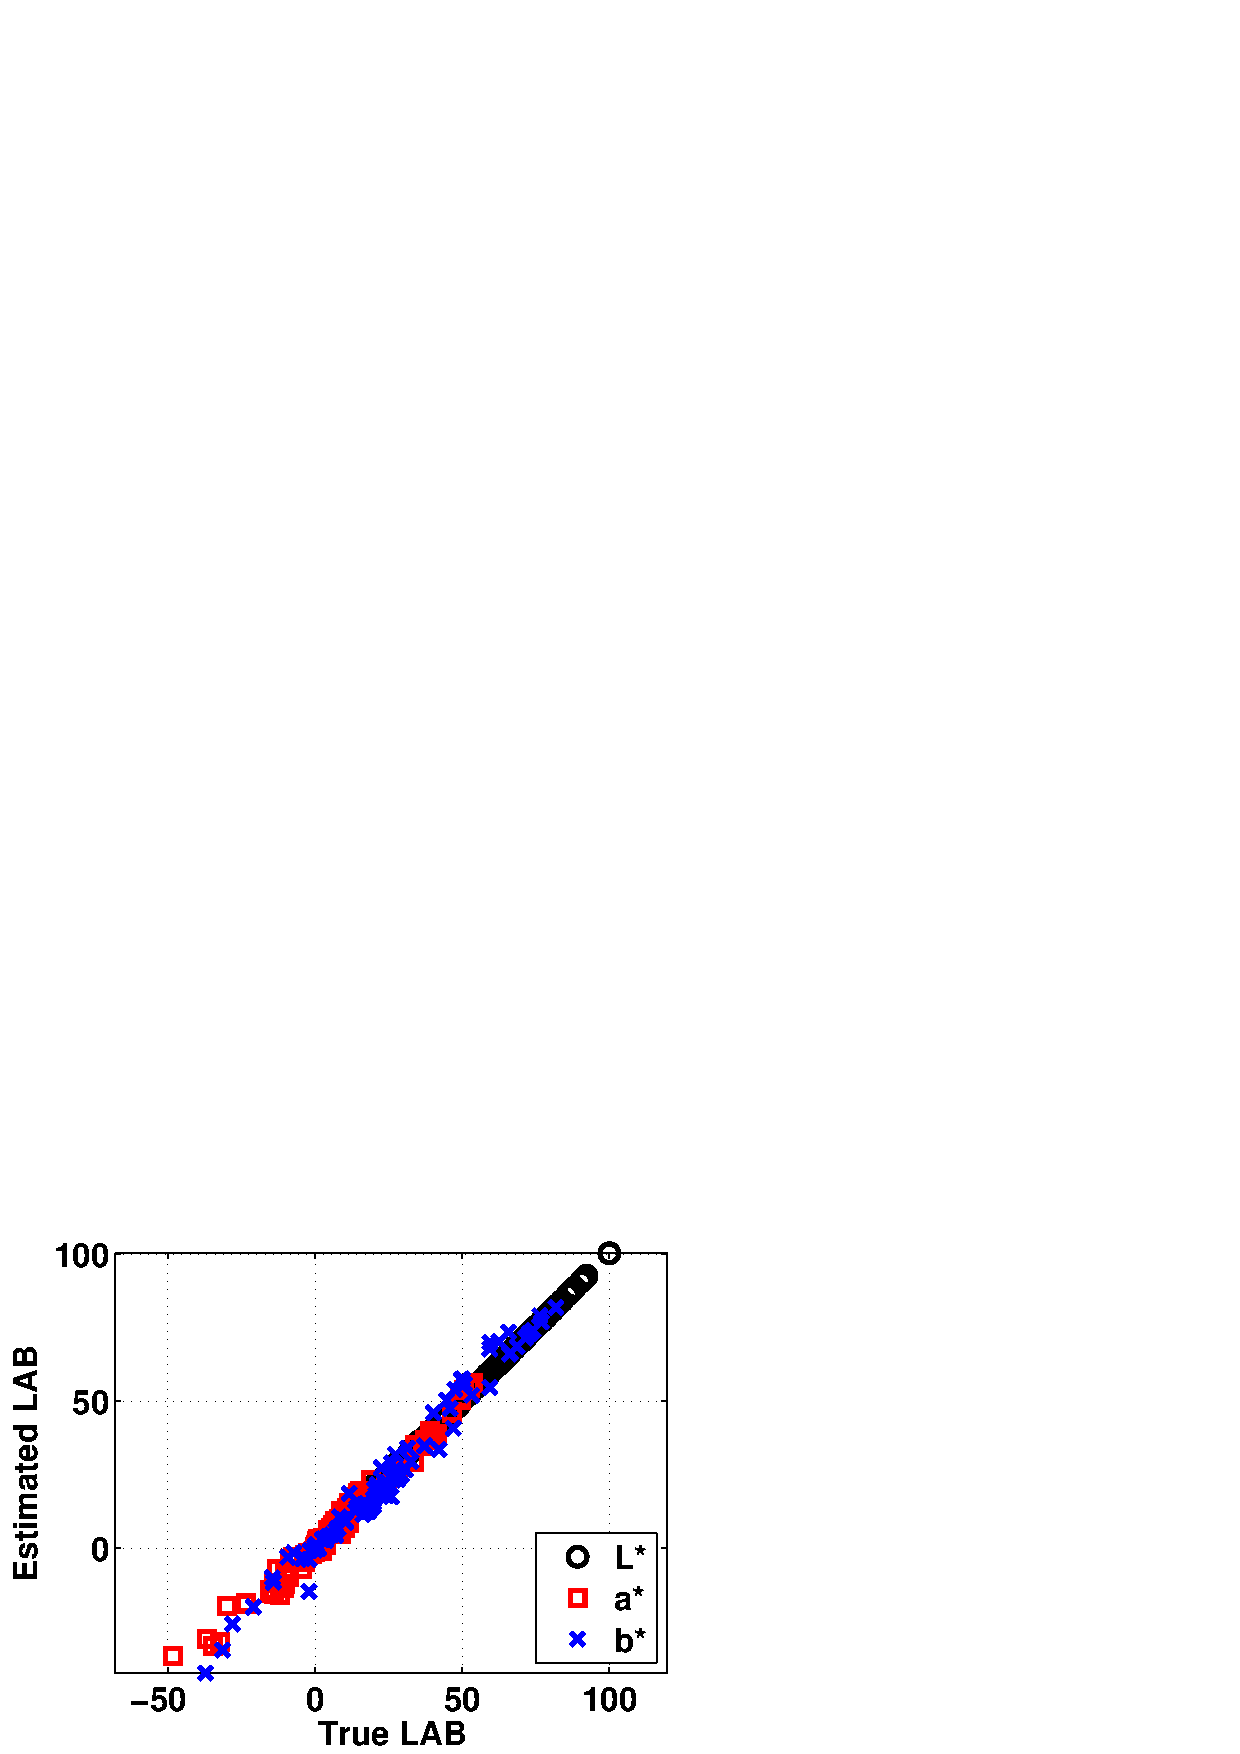
\includegraphics[width=\textwidth]{DeltaE_Tun}
    \caption{SI\_Tun+T}
\end{subfigure}
\begin{subfigure}[b]{0.325\textwidth}
    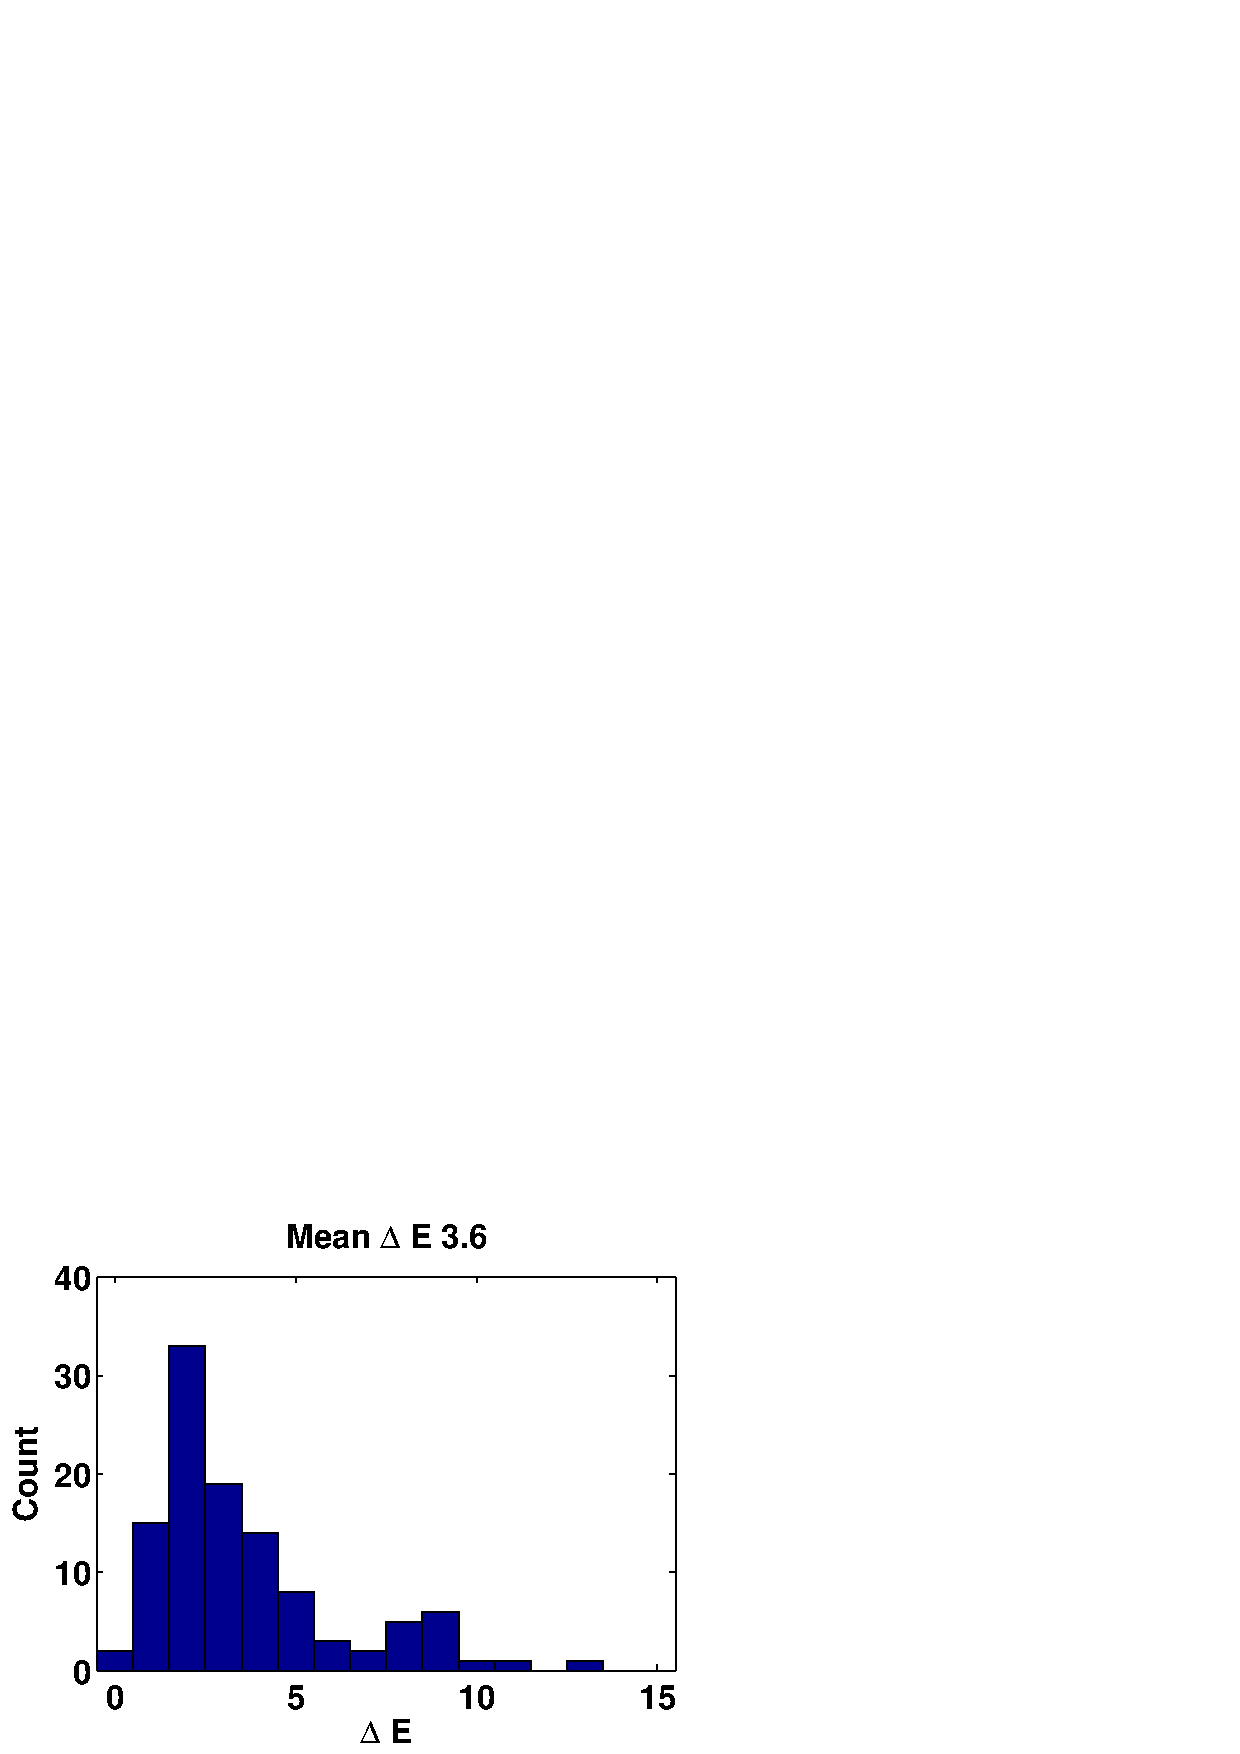
\includegraphics[width=\textwidth]{Hist_D65}
    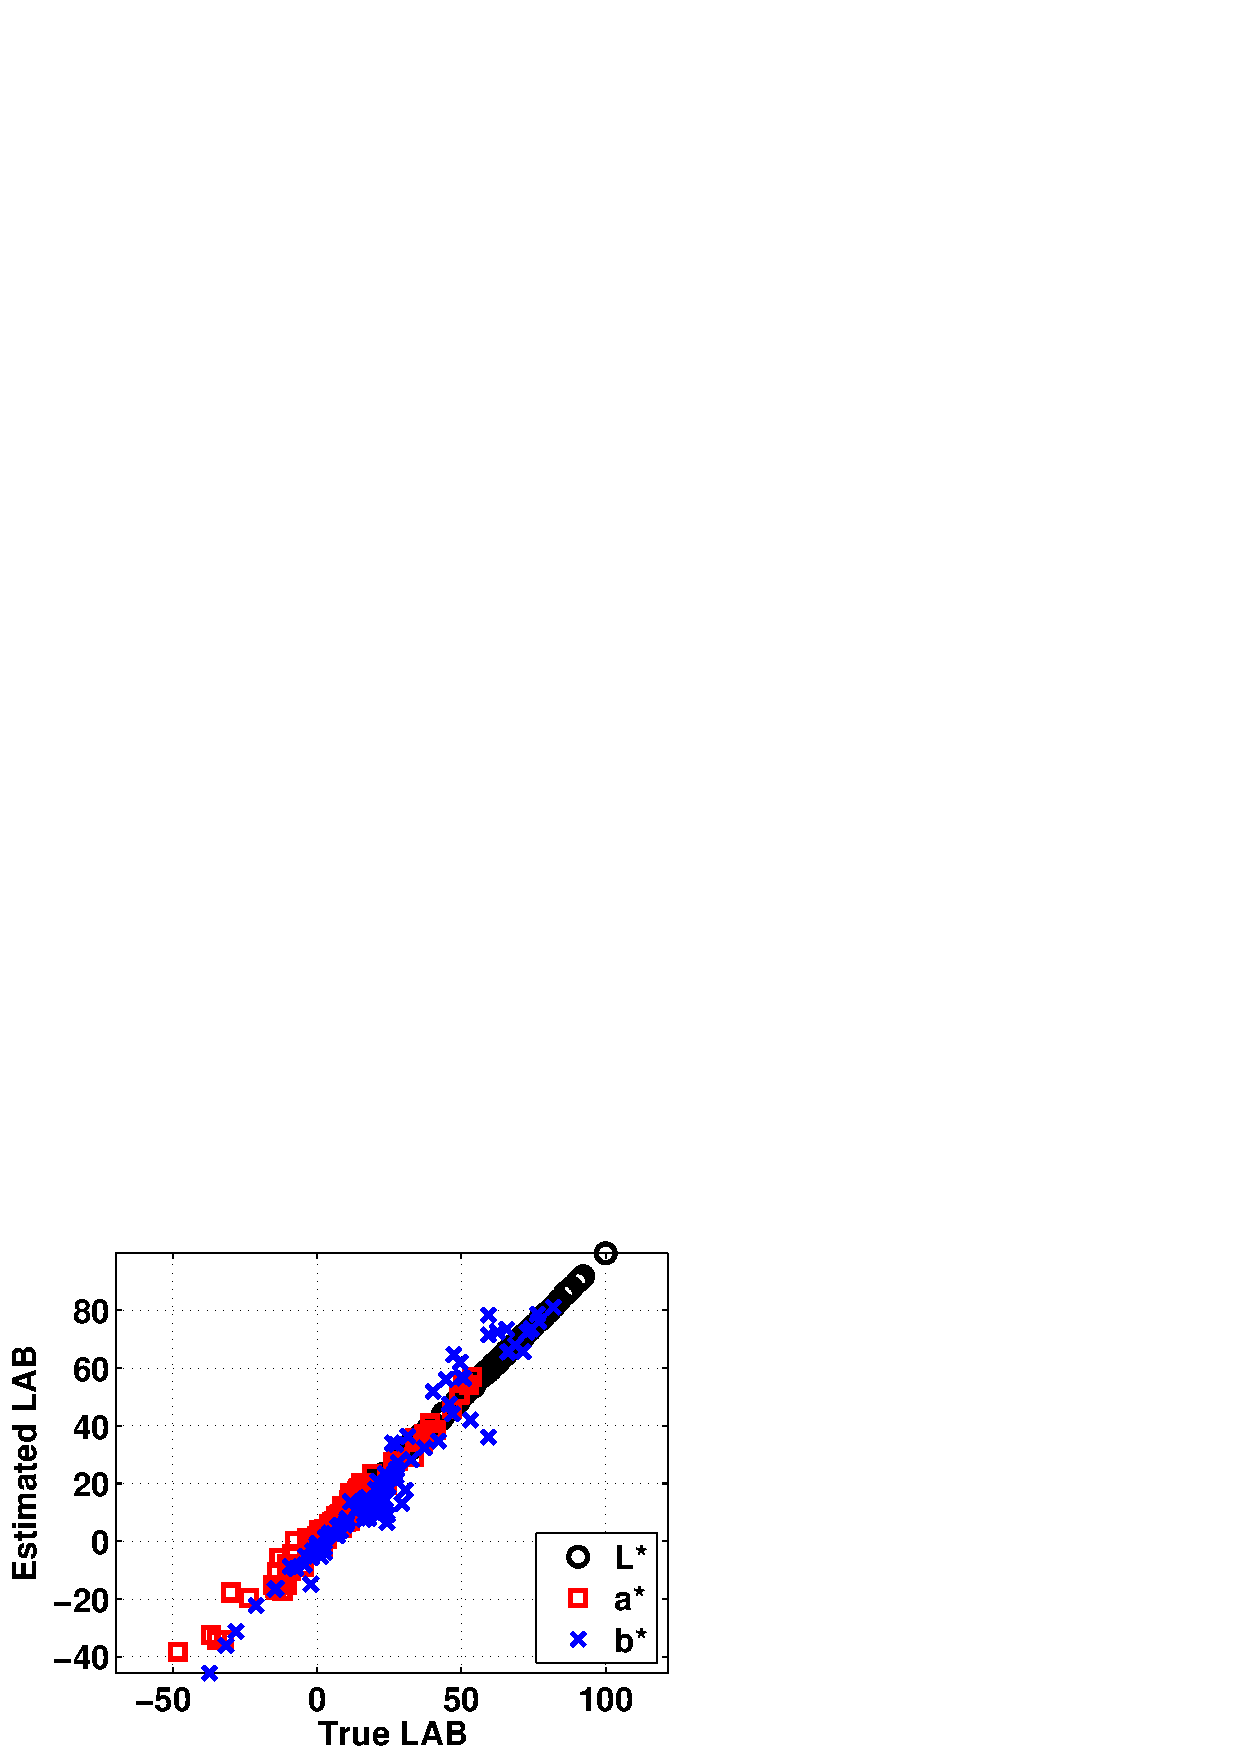
\includegraphics[width=\textwidth]{DeltaE_D65}
    \caption{SI\_D65+T}
\end{subfigure}
\caption{\textbf{Comparison of the color error distributions for a Natural-100 chart acquired under a tungsten illuminant and rendered using different L3 tables.} We compare the distribution of color reproduction error in ΔE units (top) and the comparison between true and estimated L*a*b* coordinates (bottom) for the 110 different chart reflectances for (a) the cross-illuminant table (XI), (b) the same-illuminant table for tungsten followed by the illuminant transform T (SI\_Tun+T), and (c) the same-illuminant table for D65 followed by the illuminant transform T (SI\_D65+T).}
\label{fig:colorStatisticsPlot}
\end{figure}

\begin{figure}
\begin{center}
\begin{subfigure}[b]{0.325\textwidth}
    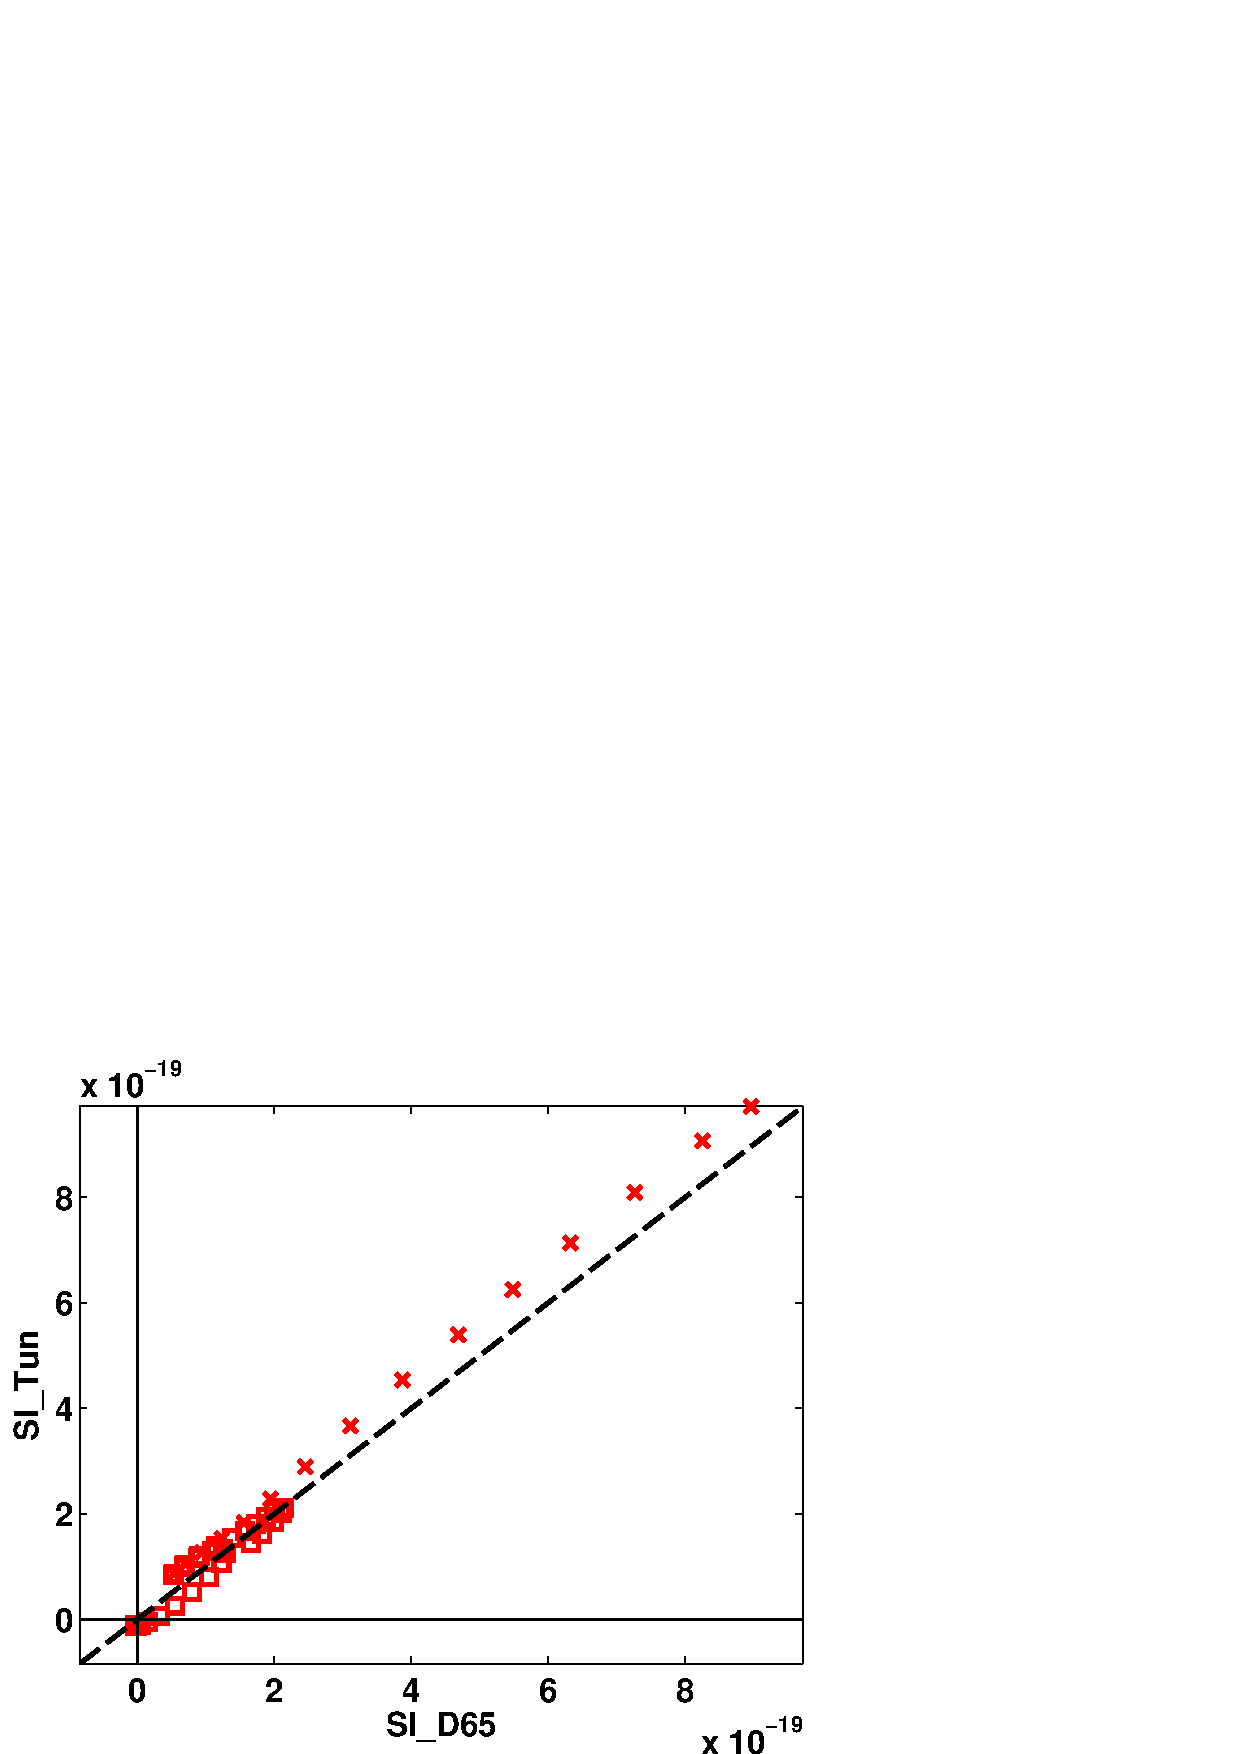
\includegraphics[width=\textwidth]{color_Statistics_r}
\end{subfigure}
\begin{subfigure}[b]{0.325\textwidth}
    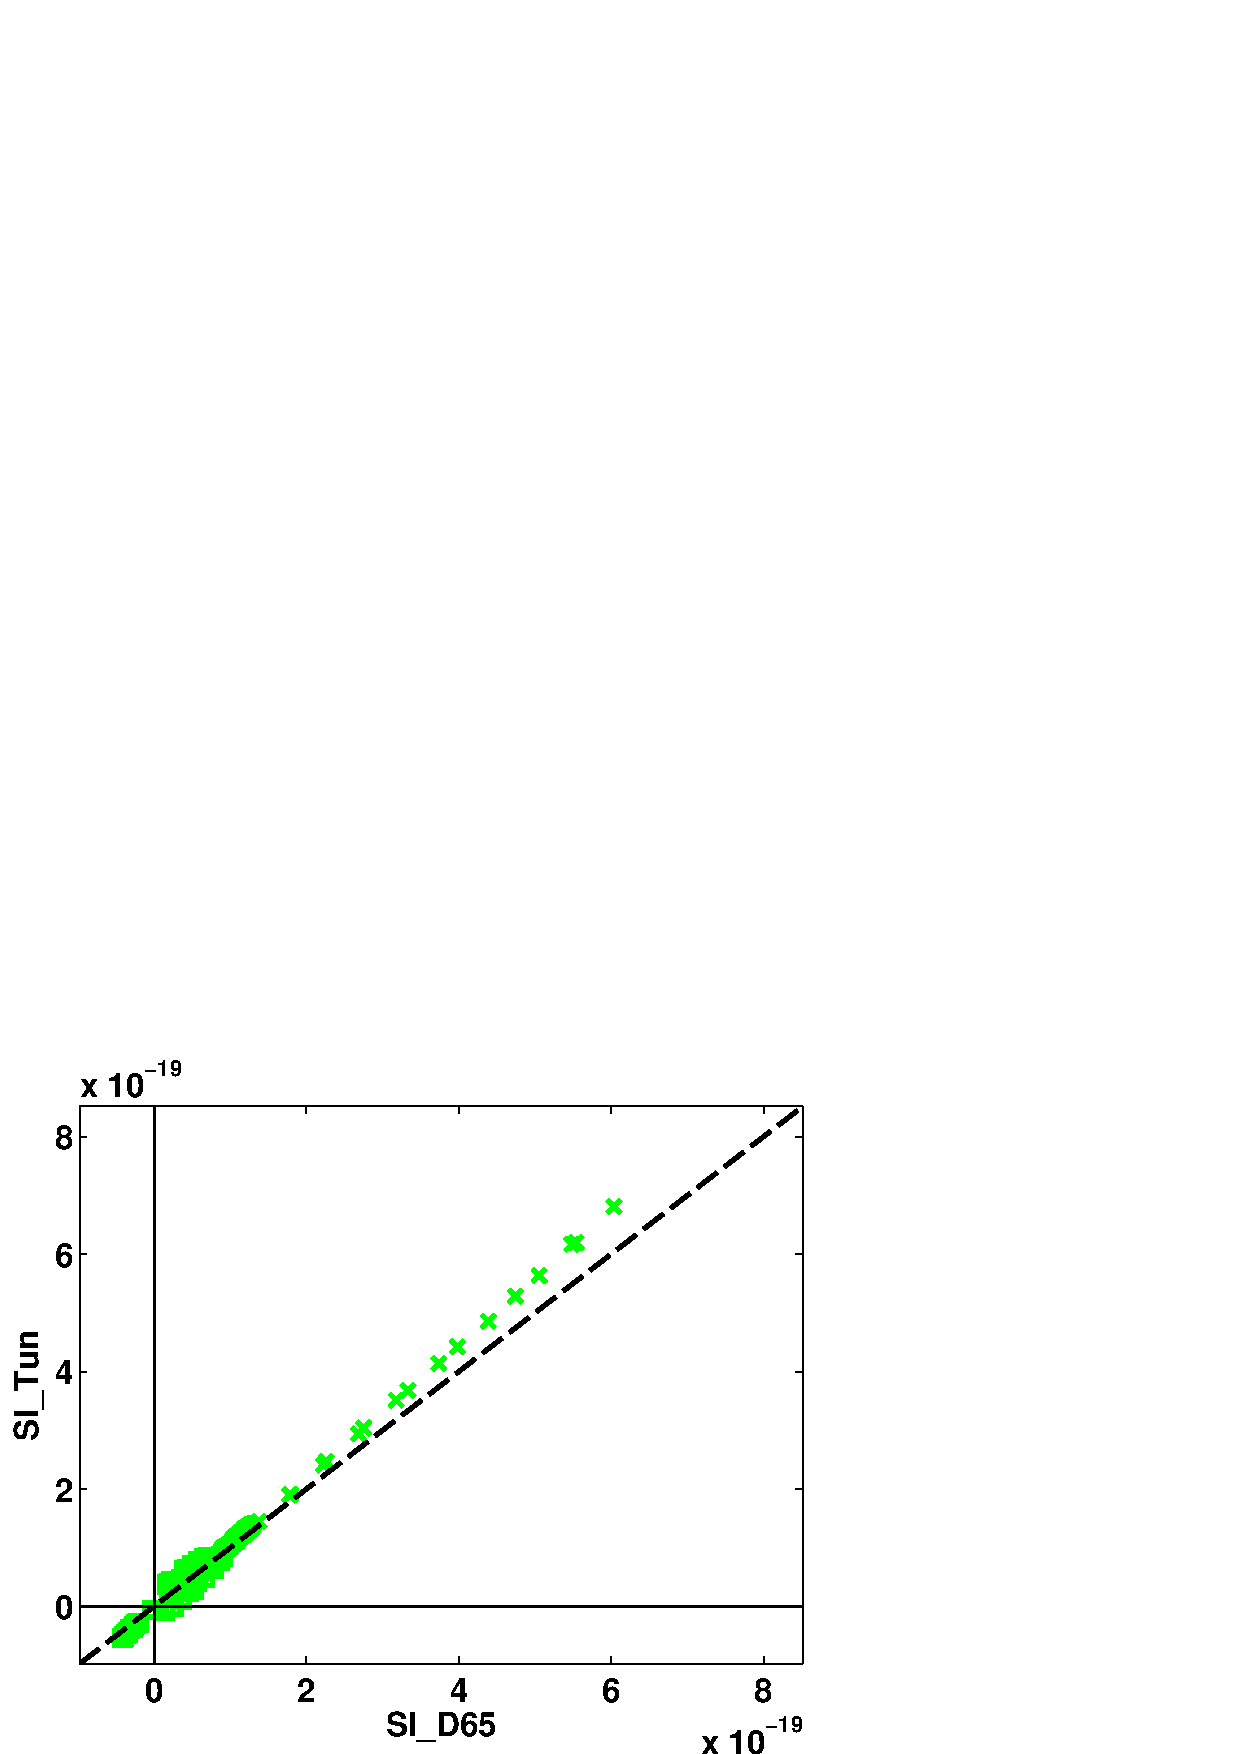
\includegraphics[width=\textwidth]{color_Statistics_g}
\end{subfigure}
\begin{subfigure}[b]{0.325\textwidth}
    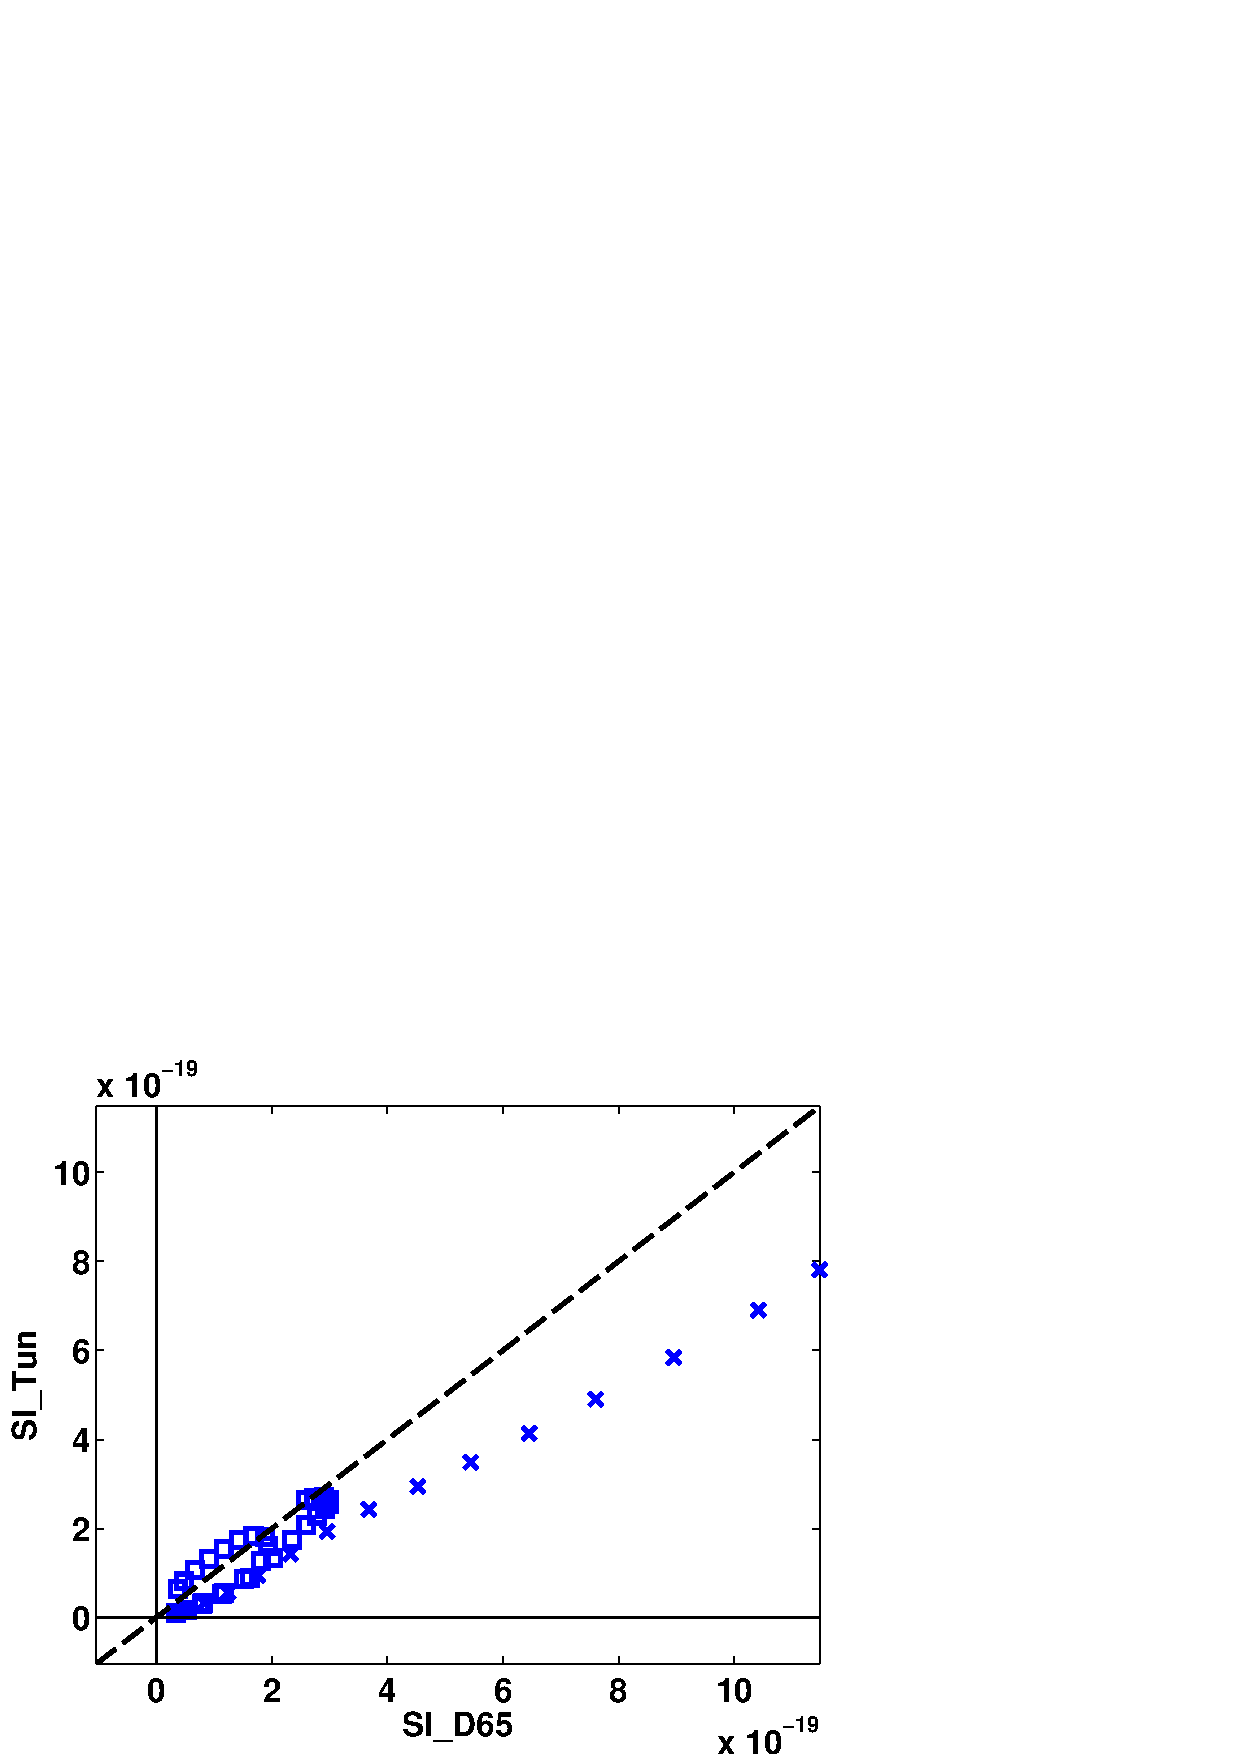
\includegraphics[width=\textwidth]{color_Statistics_b}
\end{subfigure}
\end{center}
\caption{The color statistics of the training data generate bias in the L3 same-illuminant table optimization under different illuminants.}
\label{fig:colorStatisticsPlot}
\end{figure}

\section{CONCLUSIONS}
Using a single illuminant-independent L3 table followed by a linear color correction transformation is efficient without significantly reducing color reproduction accuracy.  


% \bibliography{L3}
% \bibliographystyle{spiebib}

\end{document}
